% The frames of the results deck, shared by SLIDES_v7_2026-09-15.tex (plain) and
% SLIDES_v7_2026-09-15_annotated.tex (each slide followed by its notes). \slidenote{...}
% is defined by the wrapper: empty in the plain deck, a notes frame in the annotated one.
% \codenote{<title> [<path>:<lines>]}{slides_code/<slug>.txt} follows the notes of the slides
% that state code: empty in the plain deck, a verbatim frame of the excerpt in the annotated one
% (the excerpts and these lines come from slide_code_notes.py --write).
% Citations: [DFS21] Dick and Fernandez-Serra 2021 and the other keys of the references slide;
% [code: file:line] the repository line that implements the equation.
% Layout (2026-09-16): 37 main frames, then the Backup section of 8 frames holding the long
% tables, reached from the main frames by \hyperlink buttons; page N of the plain deck is the
% N-th frame of this file.

\begin{frame}
  \titlepage
\end{frame}
\slidenote{The deck condenses the full report (REPORT\_v7\_2026-09-15) and its summary. Two glossary slides come first, then six sections that follow the pipeline: the model (Sec. 1), the generation of the training subsets (Sec. 2, the step before any network is fitted), the pre-training of each architecture to reproduce its parent functional (Sec. 3), the optimization on the training subsets read on the training data itself (Sec. 4), the held-out generalization (Sec. 5) and the pending work (Sec. 6). The long tables sit in a Backup section after the references, reached by the buttons on the slides that summarize them. Bracketed keys cite the paper or the repository line an equation or value comes from; the keys are expanded on the references slide.}

\begin{frame}{The objects named in this talk}
  \small
  \begin{itemize}
    \item \textbf{Cell:} one trained exchange-correlation functional (an exchange and a correlation network), identified by its architecture and the number $r$ of training points it was fitted to. \textbf{Subset $r$:} the $r$ points of the 26-point DFS pool [DFS21] chosen for that column of cells (Sec. 2).
    \item \textbf{Run:} one cluster run under one configuration file; the runs differ in which architectures they train. \textbf{View:} the runs merged into one figure set. \textbf{Arm:} a run of one architecture (deep\_3x16) under a changed training protocol, shown with its tag: [25 cycles], [dpyscf parity].
    \item \textbf{Pre-training:} fitting a network to reproduce its parent functional (PBE or SCAN) before any reference data is seen. \textbf{Certificate:} the check that the clone reproduces the parent to tolerance; a failing certificate holds the group's training.
    \item \textbf{Checkpoints:} training saves the final, the lowest-training-loss and the lowest-validation-error network; every figure reads the \textbf{validation-best} one.
    \item \textbf{Rung:} the class of density variables a functional reads (GGA: density and gradient; meta-GGA: plus the kinetic-energy density; rung 3.5: plus density-matrix columns). \textbf{Start:} deep networks begin from a Glorot-initialized last layer, deep0 networks from a zeroed one, so the untrained deep0 network is the LDA.
  \end{itemize}
\end{frame}
\slidenote{These are the terms used on every later slide, gathered once. A cell is the unit of every figure and table: one column of cells is one architecture, one position along the axis is one training-subset size. The runs are cluster jobs; the view is their union, drawn once. The arms are the two variants of the density program, both on the deep\_3x16 architecture: one trains with 25 self-consistent-field cycles instead of 3, the other reproduces the DFS reference code's protocol in every setting the code can express; their cells carry a tag on the same axis as the size cells. Pre-training and its certificate are Sec. 3; the checkpoints are Sec. 4; the rungs are Sec. 1.}

\begin{frame}{The measures named in this talk}
  \small
  \begin{itemize}
    \item \textbf{WTMAD-2:} GMTKN55's weighted total mean absolute deviation of reaction energies [Goe17]: each benchmark's mean absolute error divided by its mean absolute reference value and scaled by 56.84 kcal/mol; two benchmarks are present here (BH76 barriers, W4-11 atomization energies). Lower is better; the pooled PBE value is 8.92 kcal/mol.
    \item \textbf{$\varepsilon_n$:} the DFS density error [DFS21 Eq. 20], the integrated absolute difference from the CCSD reference density per electron (PBE 0.00923). \textbf{Grid RMSE:} the root-mean-square density difference over the quadrature grid, the measure the density loss trains on.
    \item \textbf{$\mathcal{ED}$:} the harmonic mean of the energy error and $\gamma$ times the density error [DFS21 Eq. 21]; \textbf{DFS units} use $\varepsilon_n$ with $\gamma = 1084.87$ kcal/mol, \textbf{self-calibrated units} the grid RMSE with $\gamma$ set so that PBE's two legs are equal.
    \item \textbf{Beats PBE / cap:} a cell is below PBE when its $\mathcal{ED}$ is below PBE's on the same held-out slice; on the bar charts PBE's value on the cell's own slice is the black cap and a triangle marks a cell below it.
    \item \textbf{Recurring tail:} the species whose density error exceeds 1.5 times PBE's in at least half of the cells carrying them and in at least two (eight species). \textbf{T1:} the CCSD T1 diagnostic of multireference character; 38 of the 189 held-out species are above 0.02, the model-free counterpart of the tail.
  \end{itemize}
\end{frame}
\slidenote{The formal definitions are on the held-out metrics slide (Sec. 5); this slide gives the short forms so that the numbers on the way there can be read. WTMAD-2 turns errors on barriers (around 19 kcal/mol each) and on atomization energies (around 350 kcal/mol each) into comparable relative errors. The two density measures weight the density differently: the per-electron L1 measure counts every electron alike, the grid RMSE weights large local deviations more, and the two do not always agree on a cell. The combination is dominated by its smaller leg. The tail and the T1 list are the two ways of naming the species whose density comparison is least reliable: one chosen by the trained functionals' own errors, one by a property of the reference calculation.}

\begin{frame}[label=f4]{Scope}
  \small
  One network pair (exchange and correlation) per architecture and training-subset size, trained in separate cluster runs under one protocol and drawn once over every finished cell. Each run carries a pre-training, the certificate that gates its training array, and the array itself, one cell per (architecture, subset size).
  \begin{center}\footnotesize\setlength{\tabcolsep}{4pt}
  \begin{tabular}{p{2.3cm}p{6.2cm}p{4.6cm}}
  \toprule
  Run & Architectures & Cells in the figures \\ \midrule
  size & deep\_3x16, deep\_attn\_3x16, deep\_2x8, deep\_attn\_2x8 & 41 of 44 \\
  families & deep0\_3x16, deep0\_attn\_3x16, deep0\_cusp\_3x16 & 19 of 33 \\
  meta-GGA families & five SCAN-parented architectures & 0 of 55 (four FAIL, one cancelled) \\
  the two arms & deep\_3x16 [25 cycles], deep\_3x16 [dpyscf parity] & 2 of 5 each \\
  \bottomrule
  \end{tabular}
  \end{center}
  \footnotesize
  \begin{itemize}
    \item Subset sizes 1, 2, 3, 4, 5, 6, 7, 12, 15, 18, 26 points of the 26-point DFS pool [DFS21, SI Sec. II], chosen by Jensen-Shannon selection (Sec. 2).
    \item 64 cells in the figures; two evaluated cells (deep\_attn\_2x8 at 18, deep\_3x16 [25 cycles] at 15) are set aside pending re-evaluation (Sec. 6).
    \item Basis 6-311++G(3df,2pd), grid level 3, density fitting, at every stage [cfg]; the validation-best checkpoint is read for every optimization figure.
  \end{itemize}
  \hfill \hyperlink{b1}{\beamergotobutton{run table}}
\end{frame}
\slidenote{\textbf{Cell:} one trained functional, identified by its architecture and the size of the training subset it was trained on; the size run has 44 cells of which 41 are in the figures, the families run 33 of which 19, the two arms 5 each of which 2 and 2; every figure and table is drawn once over the 64 cells (the runs merged into one view). Two further cells were evaluated on the cluster but their held-out tables hold no reaction: their evaluations ran while the CCSD T1 backfill was rewriting the benchmark reference files with a key the evaluation's reference reader did not accept, so every reference was refused; both are to be re-evaluated in a later cluster session and enter the figures with the pull that follows. \textbf{Run:} a cluster run with one configuration file; the runs differ only in which architectures they train. \textbf{Pre-training:} fitting the networks to reproduce an existing functional (PBE or SCAN) before any training on reference data. \textbf{Fidelity certificate:} the check that the pre-trained networks reproduce the parent's energies to tolerance; if it fails, the group's training does not start. \textbf{Training array:} the cluster job array of cells. \textbf{DFS pool:} the training set of Dick and Fernandez-Serra's 2021 Letter. \textbf{Validation-best checkpoint:} training saves three checkpoints (final, lowest training loss, lowest validation error); the figures use the one with the lowest validation reaction-energy error. The basis, grid and density-fitting settings are those of the run configuration files (\texttt{dfs\_step7.dfs6311\_grid3\_v7*.yaml}) and are recorded in every certificate file. The run directories and the per-architecture cell counts are on the backup table.}

% =====================================================================
\section{1. Model}

\begin{frame}{1. Model: density variables and the DFS coordinates}
  With $n = n_\alpha + n_\beta$ and $\sigma = |\nabla n|^2$ [DFS21 Eqs. 4, 5]:
  \[
  k_F = (3\pi^2 n)^{1/3}, \qquad
  s = \frac{|\nabla n|}{2 k_F n}, \qquad
  r_s = \left(\frac{3}{4\pi n}\right)^{1/3},
  \]
  \[
  \zeta = \frac{n_\alpha - n_\beta}{n}, \qquad
  \phi(\zeta) = \tfrac12\left[(1+\zeta)^{4/3} + (1-\zeta)^{4/3}\right].
  \]
  The networks read logarithmic compressions of these [DFS21 Eqs. 7 to 10; code: networks.py:621--657]:
  \[
  x_0 = \ln\!\left(n^{1/3} + 10^{-5}\right), \qquad
  x_1 = \ln \phi(\zeta), \qquad
  x_s = \left(1 - e^{-s^2}\right)\ln(s + 1), \qquad
  x_\alpha = \ln\frac{\alpha + 1}{2}.
  \]
  \begin{itemize}
    \item Exchange input $[x_s, \ldots]$ with $s$ of the doubled spin channel $2 n_\sigma$ (the exchange network is evaluated per spin channel, next slides); correlation input $[x_0, x_1, x_s, \ldots]$ on the total density. The ellipsis holds the architecture's extra descriptors; on the meta-GGA rung the raw $\alpha$ is replaced by $x_\alpha$.
    \item The $10^{-5}$ in $x_0$ is the DFS reference implementation's constant [dpyscf net.py:39; code: networks.py:27].
  \end{itemize}
\end{frame}
\slidenote{$n$ is the electron density, $\sigma$ the squared gradient. $k_F$ is the Fermi wave vector of a uniform gas at density $n$; $s$ the reduced (dimensionless) density gradient, the GGA variable; $r_s$ the Wigner-Seitz radius (large where the density is low); $\zeta$ the spin polarization ($0$ closed shell, $\pm 1$ fully polarized); $\phi$ the spin-scaling factor that enters PBE correlation. The coordinates $x_0, x_1, x_s, x_\alpha$ are what the neural networks actually receive: logarithms compress the range of $n^{1/3}$ (which spans many orders of magnitude on a molecular grid) and of $s$, so that the network's inputs are of order one everywhere. $x_s$ behaves as $s^2 \ln(s+1)$ near $s = 0$ and as $\ln s$ at large $s$. The exchange network sees each spin channel separately at twice its density, which is how the exact spin-scaling relation of exchange is built in (next slides); the correlation network sees the total density and the polarization through $x_1$. The density is floored at a small cutoff before any of these variables is formed, so that the vanishing-density tail of the grid produces no infinities.}
\codenote{k\_F, s and the density floor (exchange network) [xcquinox/alec/networks.py:319--324]}{slides_code/p5_1_k_f_s_and_the_density_floor_exchange_net.txt}
\codenote{r\_s, k\_F, s (correlation network) [xcquinox/alec/networks.py:589--597]}{slides_code/p5_2_r_s_k_f_s_correlation_network.txt}
\codenote{the DFS coordinates x\_0, x\_1, x\_s (correlation network) [xcquinox/alec/networks.py:626--654]}{slides_code/p5_3_the_dfs_coordinates_x_0_x_1_x_s_correlat.txt}
\codenote{the exchange coordinate x\_s [xcquinox/alec/networks.py:341--352]}{slides_code/p5_4_the_exchange_coordinate_x_s.txt}
\codenote{the log transform and the 1e-5 constant [xcquinox/alec/networks.py:27--34]}{slides_code/p5_5_the_log_transform_and_the_1e_5_constant.txt}
\codenote{the meta-GGA coordinate ln((alpha + 1)/2) [xcquinox/alec/networks.py:48--80]}{slides_code/p5_6_the_meta_gga_coordinate_ln_alpha_1_2.txt}
\codenote{the exchange network on the doubled spin channel [xcquinox/alec/oneshot.py:465--537]}{slides_code/p5_7_the_exchange_network_on_the_doubled_spin.txt}

\begin{frame}{1. Model: the extra descriptors}
  \textbf{Iso-orbital indicator} (meta-GGA rung; SCAN's $\alpha$ [SCAN15 Eq. 2; DFS21 Eq. 6; code: metagga.py:8--9]), a contraction of the live density matrix $P$ against the AO gradients, hence self-consistent and differentiable through the SCF:
  \[
  \alpha = \frac{\tau - \tau_W}{\tau_{\rm unif}}, \qquad
  \tau = \tfrac12 \sum_i |\nabla\psi_i|^2 = \tfrac12 \sum_{\mu\nu} P_{\mu\nu}\, \nabla\chi_\mu\cdot\nabla\chi_\nu,
  \]
  \[
  \tau_W = \frac{|\nabla n|^2}{8n}, \qquad
  \tau_{\rm unif} = \tfrac{3}{10}(3\pi^2)^{2/3} n^{5/3},
  \]
  with $\alpha \ge 0$ imposed by a smooth positive part rather than a hard clip [code: metagga.py:25--31].
  \vspace{0.1em}

  \textbf{Nuclear cusp pair} (\texttt{cusp}), two bounded geometric features per grid point [code: descriptors.py:230--245]:
  \[
  x_4 = \exp(-2 Z_{\rm nearest}\, r_{\min}), \qquad
  x_5 = \tanh\!\left(\frac{1}{5}\ln \sum_A \frac{Z_A}{r_A}\right),
  \]
  $x_4$ the density-form cusp envelope $e^{-2Zr}$ [Steiner63, after Kato57], $x_5$ the log-compressed bare-nuclear potential. Both are geometric, so the synthetic pre-training mesh (Sec. 3) carries no values for them.
\end{frame}
\slidenote{$\tau$ is the (positive) kinetic-energy density of the occupied orbitals $\psi_i$; on a basis set it is a contraction of the one-particle density matrix $P$ with the gradients of the atomic-orbital functions $\chi_\mu$, which is why it can be differentiated through the self-consistent field: it depends on the live density matrix, not on a frozen reference. $\tau_W$ is the von Weizsacker kinetic-energy density, the value of $\tau$ for a single occupied orbital, and $\tau_{\rm unif}$ the value for a uniform gas at the same density. $\alpha$ therefore reads 0 in a single-orbital (one-electron or covalent bond) region, 1 in a uniform-gas-like region, and grows in regions of overlapping closed shells. The lower bound $\alpha \ge 0$ holds exactly for a single occupied orbital but can be violated numerically; a smooth positive part keeps the derivative continuous there, which a hard clip would not. The cusp pair encodes where the nuclei are: $x_4$ is 1 at a nucleus and decays with the density's own cusp envelope (the electron density falls as $e^{-2Zr}$ near a nucleus of charge $Z$, the density counterpart of Kato's wavefunction cusp condition), $x_5$ is a bounded, log-compressed version of the bare nuclear potential summed over all nuclei. Because both depend only on the geometry, the synthetic $(r_s, s, \alpha)$ mesh used to regularize pre-training has no value to give them.}
\codenote{tau from the live density matrix [xcquinox/alec/metagga.py:115--139]}{slides_code/p6_1_tau_from_the_live_density_matrix.txt}
\codenote{the smooth positive part [xcquinox/alec/metagga.py:142--152]}{slides_code/p6_2_the_smooth_positive_part.txt}
\codenote{alpha = (tau - tau\_W) / tau\_unif [xcquinox/alec/metagga.py:163--274]}{slides_code/p6_3_alpha_tau_tau_w_tau_unif.txt}
\codenote{the alpha descriptor of the network input [xcquinox/alec/descriptors.py:432--472]}{slides_code/p6_4_the_alpha_descriptor_of_the_network_inpu.txt}
\codenote{the cusp pair x\_4, x\_5 [xcquinox/alec/descriptors.py:225--258]}{slides_code/p6_5_the_cusp_pair_x_4_x_5.txt}

\begin{frame}{1. Model: the network}
  \small
  Each of the exchange and the correlation networks is a multilayer perceptron of \texttt{depth} hidden layers of \texttt{nodes} units with GELU activations, read at every grid point; its scalar output $g$ becomes the enhancement factor on the next slide [code: networks.py:169, 379--404].
  \begin{itemize}
    \item \textbf{GELU:} $\mathrm{GELU}(z) = z\,\Phi(z)$ with $\Phi$ the standard normal distribution function, a smooth rectifier; the enhancement factors and their derivatives (the potential) are smooth in the density variables.
    \item \textbf{Last layer:} Glorot-initialized in the deep networks, zeroed in the deep0 networks, so the latter start exactly at $F = 1$ (the LDA) before pre-training.
    \item \textbf{Attention variants} (\texttt{\_attn}) [Vas17 Eq. 1; Xio20; code: net.py:55--136]: after the first hidden layer, the $H$ hidden units are $h$ tokens of dimension $d_k = H/h$ under pre-layer-norm self-attention across the token axis, a per-point re-mixing of hidden units; the functional stays semilocal.
  \end{itemize}
  \[
  \mathrm{Attn}(Q, K, V) = \mathrm{softmax}\!\left(\frac{QK^{\top}}{\sqrt{d_k}}\right) V, \qquad
  x \leftarrow x + W^{O}\,\mathrm{Concat}(\mathrm{head}_1, \ldots, \mathrm{head}_h)(\mathrm{LN}(x)).
  \]
\end{frame}
\slidenote{The networks are small: 3 hidden layers of 16 units (the 3x16 architectures) or 2 of 8 (the 2x8 pair), evaluated independently at every quadrature point of the molecular grid. GELU is the Gaussian error linear unit; unlike the ReLU it has a continuous derivative, which matters because the exchange-correlation potential entering the self-consistent field is the functional derivative of the energy and inherits the activation's smoothness. The attention variants insert one self-attention block after the first hidden layer: the hidden vector at a grid point is cut into $h$ tokens (4 for the 3x16 networks, 2 for the 2x8 pair), each token attends to the others with the standard scaled dot-product formula, and the result is added back (a residual) after a layer normalization. It re-mixes hidden units at one grid point; it does not look at neighbouring points, so the functional stays semilocal.}
\codenote{the MLP, GELU, the attention block after the first hidden layer, the gate and the output [xcquinox/alec/networks.py:366--405]}{slides_code/p7_1_the_mlp_gelu_the_attention_block_after_t.txt}
\codenote{the network construction and the zero-initialized last layer [xcquinox/alec/networks.py:283--300]}{slides_code/p7_2_the_network_construction_and_the_zero_in.txt}
\codenote{the self-attention block [xcquinox/net.py:50--136]}{slides_code/p7_3_the_self_attention_block.txt}

\begin{frame}{1. Model: the functional form}
  \small
  MLP output $g$ at a grid point:
  \[
  F_x = 1 + \mathcal{L}_{1.804}\!\left(G_x \cdot g_x\right), \qquad
  F_c = 1 + \mathcal{L}_{2}\!\left(G_c \cdot g_c\right),
  \]
  \[
  \mathcal{L}_{\lambda}(z) = \lambda\,\mathrm{sigmoid}\!\left(z - \ln(\lambda - 1)\right) - 1 \quad \text{[DFS21 Eq. 11]},
  \]
  \[
  G = \tanh^2(s) \ \ \text{(GGA)}, \qquad G = x_s + \tanh^2(x_\alpha) \ \ \text{(meta-GGA) [DFS21 Eq. 12]}.
  \]
  $\mathcal{L}_\lambda(0) = 0$ and $F \in (0, \lambda)$; $\lambda = 1.804 = 1 + \kappa_{\rm PBE}$ for exchange [PBE96 Eq. 14] (DFS uses 1.174 [PRSB14]), $\lambda = 2$ so that $F_c \ge 0$ [DFS21 Eq. 13]. The gate $G$ pins $F = 1$ where the gradient vanishes.
  \[
  E_{xc} = \tfrac12\left(E_x[2 n_\alpha] + E_x[2 n_\beta]\right) + E_c[n_\alpha, n_\beta] \ \ \text{[OP79; code: descriptors.py:124]},
  \]
  \[
  E_x[n] = \int n\, \epsilon_x^{\rm LDA}(n)\, F_x\, d^3r, \qquad
  E_c = \int n\, \epsilon_c^{\rm PW92}(r_s, \zeta)\, F_c\, d^3r \ \ \text{[PW92]}.
  \]
\end{frame}
\slidenote{The functional is written as the local density approximation times an enhancement factor: $E_x = \int n\,\epsilon_x^{\rm LDA}(n) F_x$ for exchange and the same with the PW92 uniform-gas correlation energy per particle for correlation. $F_x = F_c = 1$ is the LDA; PBE, SCAN and the trained networks differ in how $F$ depends on the density variables. The network's raw output $g$ is passed through the bounded map $\mathcal{L}_\lambda$, which sends 0 to 0 and confines $F$ to $(0, \lambda)$; for exchange $\lambda = 1.804$ is the PBE ceiling derived from the Lieb-Oxford bound, for correlation $\lambda = 2$ merely guarantees $F_c \ge 0$ (the upper value is not used). The gate $G$ multiplies the network output by $\tanh^2(s)$, which vanishes where the gradient vanishes, so the uniform electron gas limit $F = 1$ is exact by construction; on the meta-GGA rung the DFS gate adds a term in $x_\alpha$. The exchange energy is assembled from the exact spin-scaling relation of Oliver and Perdew: exchange of a spin-polarized system is the average of the spin-unpolarized functional evaluated at twice each spin density; this is why the exchange network is evaluated per spin channel.}
\codenote{the bounded map L\_lambda [xcquinox/alec/networks.py:129--169]}{slides_code/p8_1_the_bounded_map_l_lambda.txt}
\codenote{the exchange and correlation energy densities (LDA and PW92 factors) [xcquinox/alec/models.py:175--215]}{slides_code/p8_2_the_exchange_and_correlation_energy_dens.txt}
\codenote{the spin-scaled exchange energy (Oliver and Perdew) [xcquinox/alec/oneshot.py:465--537]}{slides_code/p8_3_the_spin_scaled_exchange_energy_oliver_a.txt}

\begin{frame}[label=f9]{1. Model: the architectures}
  \begin{center}\small
  \begin{tabular}{llllll}
  \toprule
  Architecture & Last layer & Rung, parent & Hidden & Heads & Extra \\ \midrule
  deep\_3x16 & Glorot & GGA, PBE & 3 x 16 & none & none \\
  deep\_attn\_3x16 & Glorot & GGA, PBE & 3 x 16 & 4 & none \\
  deep0\_3x16 & zeroed & GGA, PBE & 3 x 16 & none & none \\
  deep0\_attn\_3x16 & zeroed & GGA, PBE & 3 x 16 & 4 & none \\
  \bottomrule
  \end{tabular}
  \end{center}
  \small
  \begin{itemize}
    \item Inputs: $F_x$ from $x_s$, $F_c$ from $x_0, x_1, x_s$; the cusp architectures add $x_4, x_5$ to both, the meta-GGA ones $x_\alpha$ as well, the rung-3.5 ones their occupancy columns.
    \item The 2x8 pair, deep\_2x8 and deep\_attn\_2x8 (2 heads), are the same GGA networks at 2 x 8; the arms' cells are deep\_3x16 trained under the 25-cycle and the dpyscf-parity protocol, shown on the same axis as deep\_3x16 [25 cycles] and deep\_3x16 [dpyscf parity].
    \item deep\_3x16 and deep0\_3x16 have the same layers, inputs and parameter count and differ only in the start; after pre-training both are PBE clones, so the two columns are replicates of one architecture under two starts: their combined held-out verdicts agree at every subset size (Sec. 5).
  \end{itemize}
  \hfill \hyperlink{b2}{\beamergotobutton{all eleven}}
\end{frame}
\slidenote{\textbf{The names:} the family word states the initialization of the last layer (deep: Glorot; deep0: zeroed, so pre-training starts from the LDA), then the descriptor and attention tokens, then the size. \textbf{Why deep\_3x16 and deep0\_3x16 look alike:} both are depth 3, width 16 with the same inputs and the same parameter count; the one difference is the start. In deep0\_3x16 the last layer's weights and bias start at zero, so the untrained network returns exactly the LDA ($F = 1$), whereas deep\_3x16 starts from a Glorot initialization. Pre-training then fits both to PBE; the certificate shows both pass (deep\_3x16 mean $|\Delta AE|$ 0.162, deep0\_3x16 0.114 kcal/mol). \textbf{Do the deep networks do worse?} No: deep0\_3x16 and deep\_3x16 are below PBE on the combined objective at the same subset sizes (1, 7, 12, 15, 18, 26) and above it at the same sizes (2 to 6); on energy alone deep0\_3x16 is below PBE at 3 and 4 points where deep\_3x16 is not. The comparison is between two clones of one architecture, which is a replicate rather than an architecture contrast. The descriptor families (cusp, meta-GGA, rung 3.5; the backup table) are the actual architecture axes, and their cells are still queued or held.}
\codenote{the architecture record [xcquinox/alec/config.py:103--159]}{slides_code/p9_1_the_architecture_record.txt}
\codenote{the registry entries shallow, shallow\_attn, medium and medium\_attn (shown deep\_2x8, deep\_attn\_2x8, deep\_3x16, deep\_attn\_3x16) [xcquinox/alec/config.py:512--515]}{slides_code/p9_2_the_registry_entries_shallow_shallow_att.txt}
\codenote{the registry entries deep\_3x16, deep\_attn\_3x16, deep\_cusp\_3x16 (shown deep0\_*) [xcquinox/alec/config.py:579--592]}{slides_code/p9_3_the_registry_entries_deep_3x16_deep_attn.txt}
\codenote{the registry entry deep\_cusp\_mgga\_3x16 [xcquinox/alec/config.py:691--695]}{slides_code/p9_4_the_registry_entry_deep_cusp_mgga_3x16.txt}
\codenote{from\_spec: the fields an entry sets [xcquinox/alec/config.py:385--470]}{slides_code/p9_5_from_spec_the_fields_an_entry_sets.txt}

% =====================================================================
\section{2. Training-subset generation}

\begin{frame}[label=f10]{2. Subsets: the 26-point DFS pool [DFS21 SI Sec. II]}
  \small
  \begin{itemize}
    \item 21 atomization energies (G2/97 molecules), 3 BH76 reaction energies and 2 IP13 ionization potentials: the training set of the Letter, 26 points over 30 unique species.
    \item Each point carries the species its loss term needs: an atomization its molecule and the H and Li anchors it contains, a reaction every reactant and product, an ionization the neutral and the cation.
    \item References: atomization energies [HK12] with H2O and C2H2 from [W411]; reaction energies [Goe17, BH76RC]; ionization potentials [NIST]. Code: dfs\_pool.py, training\_points.py:347--420.
    \item The pool is indexed 0 to 25 in the selection ledger; the chosen subsets of the next slides are lists of these indices.
  \end{itemize}
  \hfill \hyperlink{b3}{\beamergotobutton{the 26 points}}
\end{frame}
\slidenote{\textbf{Point:} one unit of training signal with a reference value: an atomization energy (the energy to break a molecule into its atoms), a reaction energy, or an ionization potential. \textbf{Species:} the molecules and atoms whose self-consistent energies the point's loss needs; an atomization energy needs the molecule and its atoms, but only the H and Li atoms are attached to the point as anchors because those are the atomic densities the DFS training set included; the other free atoms enter through the atom-anchor channel (Sec. 4). \textbf{Idx} is the index in the selection ledger; the chosen subsets on the later slide are lists of these indices. The pool reproduces the training set of the DFS Letter: 21 of its 22 G2/97 molecules as atomization energies, the three BH76 barrier reactions and the two ionization potentials; the reference values are the non-relativistic, zero-point-exclusive atomization energies of Haunschild and Klopper (two taken from W4-11), the GMTKN55 BH76RC reaction energies and NIST ionization potentials. The full table, with every species' charge and spin, is on the backup slide.}
\codenote{the 21 atomization points (names, spins, charges, references) [xcquinox/alec/dfs\_pool.py:106--225]}{slides_code/p10_1_the_21_atomization_points_names_spins_ch.txt}
\codenote{the three BH76 reaction points [xcquinox/alec/dfs\_pool.py:308--397]}{slides_code/p10_2_the_three_bh76_reaction_points.txt}
\codenote{the two ionization points [xcquinox/alec/dfs\_pool.py:427--466]}{slides_code/p10_3_the_two_ionization_points.txt}
\codenote{the H and Li anchors [xcquinox/alec/dfs\_pool.py:472--477]}{slides_code/p10_4_the_h_and_li_anchors.txt}
\codenote{the pool assembly [xcquinox/alec/dfs\_pool.py:547--639]}{slides_code/p10_5_the_pool_assembly.txt}
\codenote{the 26 points and their species [xcquinox/alec/training\_points.py:347--436]}{slides_code/p10_6_the_26_points_and_their_species.txt}

\begin{frame}{2. Subsets: the descriptor distributions}
  \small
  One PBE SCF per species (def2-SVP, grid level 1) [code: subset\_selection.py:106--118, 448--470] gives at every grid point $g$ with quadrature weight $w_g$
  \[
  \rho^{1/3}, \qquad
  s = \frac{|\nabla \rho|}{2 (3\pi^2)^{1/3} \rho^{4/3}} \ \ \text{[PBE96]}, \qquad
  \alpha = \frac{\tau - \tau_W}{\tau_{\rm unif}} \ \ \text{[SCAN15], clipped to } [0, 100].
  \]
  A point's sample is the concatenation of its species' grid points; the reference is the concatenation over all 26 points. Each marginal is binned into 200 equal-width bins between its 0.1 and 99.9 percentiles and normalized to a mass function:
  \[
  h_x^{(b)} = \sum_{g \,:\, x_g \in \text{bin } b} w_g, \qquad P_x^{(b)} = \frac{h_x^{(b)}}{\sum_{b'} h_x^{(b')}} .
  \]
  \begin{center}
  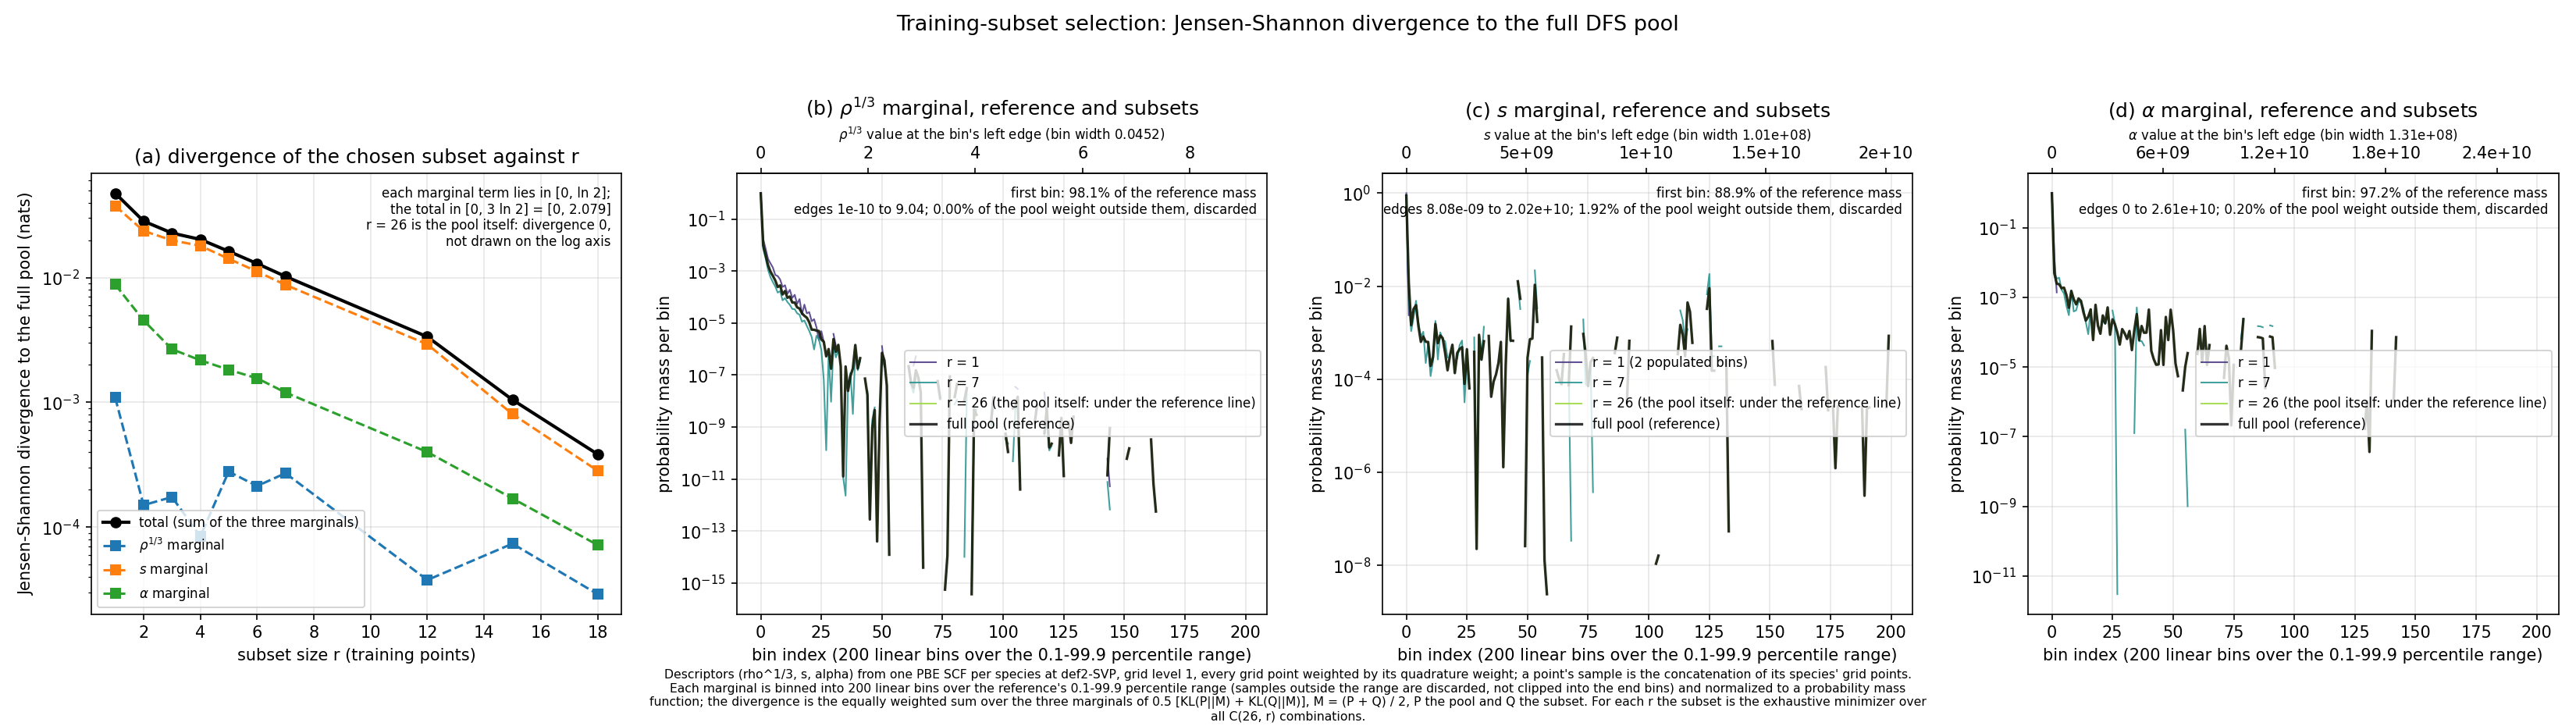
\includegraphics[width=0.72\linewidth]{figures_dfs_step7_v7_subsets/subset_jsd_vs_full.png}
  \end{center}
\end{frame}
\slidenote{The idea of the selection is to pick, for each subset size, the subset of training points whose electron densities look most like the whole pool in the variables a GGA or meta-GGA functional sees. Those variables are $\rho^{1/3}$ (the density, compressed), $s$ (the reduced gradient) and $\alpha$ (the iso-orbital indicator); they are computed once per species from a cheap PBE calculation on a small basis and a coarse grid, at every quadrature point of that species' grid. \textbf{Marginal:} the one-dimensional distribution of one of the three variables. \textbf{Histogram and mass function:} the range of each variable between its 0.1th and 99.9th percentile over the whole pool is cut into 200 equal bins; each grid point adds its quadrature weight to the bin its value falls in, and the histogram is normalized to sum to one, so that it is a probability mass function independent of the number of grid points or of the bin width. \textbf{The figure:} left, the divergence of the chosen subset from the pool against the subset size (total and the three marginal terms, log scale; the full pool has divergence zero and is not drawn on a log axis); right, the three reference mass functions (black) with the subsets at 1, 7 and 26 points overlaid, against the bin index, with the bin's variable value on the upper axis. The first bin dominates each marginal; the reasons are on the next slide.}
\codenote{the descriptor triple (rho\^{}(1/3), s, alpha) and the clip to [0, 100] [xcquinox/alec/subset\_selection.py:81--119]}{slides_code/p11_1_the_descriptor_triple_rho_1_3_s_alpha_an.txt}
\codenote{one PBE SCF per species at def2-svp, grid level 1 [xcquinox/alec/subset\_selection.py:375--406]}{slides_code/p11_2_one_pbe_scf_per_species_at_def2_svp_grid.txt}
\codenote{a point's sample is the concatenation over its species [xcquinox/alec/subset\_selection.py:409--445]}{slides_code/p11_3_a_point_s_sample_is_the_concatenation_ov.txt}
\codenote{the reference histograms: 200 bins between the 0.1 and 99.9 percentiles [xcquinox/alec/subset\_selection.py:448--469]}{slides_code/p11_4_the_reference_histograms_200_bins_betwee.txt}
\codenote{binning with the shared edges and the mass function [xcquinox/alec/subset\_selection.py:175--193]}{slides_code/p11_5_binning_with_the_shared_edges_and_the_ma.txt}
\codenote{binning with the shared edges [xcquinox/alec/subset\_selection.py:248--259]}{slides_code/p11_6_binning_with_the_shared_edges.txt}

\begin{frame}{2. Subsets: the metric [Lin91]}
  \small
  The distance between a candidate subset $S$ and the pool is the Jensen-Shannon divergence [code: subset\_selection.py:213--246, 472] summed over the three marginals with equal weights, $P_x$ the pool and $Q_x$ the subset mass function, probabilities floored at $10^{-12}$, natural logarithm:
  \[
  \mathrm{JSD}(S) = \sum_{x \in \{\rho^{1/3},\, s,\, \alpha\}} \tfrac12 \left[ \mathrm{KL}(P_x \,\|\, M_x) + \mathrm{KL}(Q_x \,\|\, M_x) \right], \qquad
  M_x = \tfrac12 (P_x + Q_x),
  \]
  \[
  \mathrm{KL}(P \,\|\, Q) = \sum_b P^{(b)} \ln \frac{P^{(b)}}{Q^{(b)}}, \qquad \text{each marginal term in } [0, \ln 2].
  \]
  \begin{itemize}
    \item The linear edges reach the low-density tails ($s$ to $2.0\times10^{10}$, $\alpha$ to $2.6\times10^{10}$, $\rho^{1/3}$ from $10^{-10}$ to 9.04), so the first bin holds 98.1, 88.9 and 97.2 percent of the weighted reference mass: the whole chemical range for $s$ and $\alpha$, the vacuum tail ($\rho < 9.2\times10^{-5}$) for $\rho^{1/3}$.
    \item The metric therefore compares the low-density tails of the molecular grids ($s$, $\alpha$) and the valence and core region ($\rho^{1/3}$); the $s$ term is 74 to 89 percent of every divergence.
  \end{itemize}
\end{frame}
\slidenote{\textbf{Kullback-Leibler divergence} $\mathrm{KL}(P\|Q)$ measures how different a distribution $P$ is from $Q$; it is zero when they coincide and is not symmetric. \textbf{Jensen-Shannon divergence} is its symmetrized, bounded form: each distribution is compared with the average $M$ of the two, so it is symmetric and, with the natural logarithm, lies between 0 and $\ln 2$ per marginal; the three marginals are summed with equal weight, so the total lies between 0 and $3\ln 2 = 2.08$. "Natural logarithm" is what the report's "in nats" meant: a nat is the unit of information when logarithms are natural rather than base 2 (bits); the choice only scales the numbers. The $10^{-12}$ floor avoids $\ln 0$ in empty bins. \textbf{Why the first bin dominates:} the bin edges are linear over the 0.1 to 99.9 percentile range, and on a molecular quadrature grid the low-density tail carries enormous $s$ and $\alpha$ values (the density falls exponentially while its gradient and kinetic terms do not fall as fast), so the range stretches to $10^{10}$ and the whole chemically relevant range of $s$ and $\alpha$ ($s \lesssim 5$, $\alpha \lesssim 10$) falls in bin 0; for $\rho^{1/3}$ the opposite holds: bin 0 covers only $\rho < 9.2\times10^{-5}$ (vacuum), and the valence and core densities occupy the higher bins. The metric therefore compares subsets mainly on how their grids' low-density tails are distributed, which is a property of the selection as it was run and is stated rather than changed here because every trained cell used these subsets.}
\codenote{the probability floor 1e-12 [xcquinox/alec/subset\_selection.py:54--54]}{slides_code/p12_1_the_probability_floor_1e_12.txt}
\codenote{the Kullback-Leibler term [xcquinox/alec/subset\_selection.py:196--210]}{slides_code/p12_2_the_kullback_leibler_term.txt}
\codenote{the Jensen-Shannon divergence over the three marginals [xcquinox/alec/subset\_selection.py:213--245]}{slides_code/p12_3_the_jensen_shannon_divergence_over_the_t.txt}

\begin{frame}{2. Subsets: the search}
  \small
  \begin{itemize}
    \item For each $r \in \{1,\ldots,7, 12, 15, 18, 26\}$ the subset is the exhaustive minimizer of $\mathrm{JSD}(S)$ over all $\binom{26}{r}$ combinations: 26 candidates at $r = 1$, 9.7 million at $r = 12$, one at $r = 26$ (the whole pool).
    \item Histograms add over disjoint samples, so every point's histogram is binned once and a candidate's mass function is a sum; a candidate with no grid point inside a marginal's range gets an infinite divergence and is never chosen.
    \item The subsets are nested only where the minimizer happens to nest: the 2-to-6-point subsets are barriers and ionizations with one or two molecules; from seven points on, atomization energies dominate (next slide).
    \item The L2 distance was computed and stored beside the JSD but no training run used it.
  \end{itemize}
\end{frame}
\slidenote{\textbf{The search} is exhaustive: every subset of size $r$ is scored, using the fact that histograms add over disjoint samples so the per-point histograms are pre-binned once; at twelve points that is 9.7 million candidates, each scored as a sum of pre-binned histograms and one divergence evaluation. The infinite-divergence rule removes candidates whose grids never reach one of the three marginals' ranges; in practice every candidate reaches them. Nesting is not imposed: the best seven-point subset need not contain the best six-point subset, and it does not (the slide after next lists them). The composition of the small subsets, barriers and ionizations rather than molecules, follows from the metric: a barrier reaction contributes four or five species' grids and covers more of the pool's descriptor distribution than a single molecule.}
\codenote{the exhaustive search over C(26, r) [xcquinox/alec/subset\_selection.py:472--688]}{slides_code/p13_1_the_exhaustive_search_over_c_26_r.txt}

\begin{frame}[label=f14]{2. Subsets: the chosen subsets [ledger subset\_index\_log.json; plot\_subset\_jsd.py]}
  \begin{center}\footnotesize\setlength{\tabcolsep}{3pt}
  \begin{tabular}{rp{5.8cm}lllll}
  \toprule
  $r$ & Points (ledger index order) & AE / BH76 / IP & JSD & $\rho^{1/3}$ & $s$ & $\alpha$ \\ \midrule
  1 & H2O & 1 / 0 / 0 & 0.0475 & 0.00109 & 0.03764 & 0.00881 \\
  7 & CHN, CO2, HLi, CH, OH+N2\_to\_H+N2O, Li\_IP, C\_IP & 4 / 1 / 2 & 0.0102 & 0.00027 & 0.00877 & 0.00120 \\
  12 & CO2, C2H2, CO, HLi, CH, NO2, CH2, OH+N2\_to\_H+N2O, OH+CH3\_to\_O+CH4, HF+F\_to\_H+F2, Li\_IP, C\_IP & 7 / 3 / 2 & 0.0034 & 0.00004 & 0.00292 & 0.00040 \\
  26 & the whole pool & 21 / 3 / 2 & 0 & 0 & 0 & 0 \\
  \bottomrule
  \end{tabular}
  \end{center}
  \small
  \begin{itemize}
    \item The $\rho^{1/3}$, $s$ and $\alpha$ columns are the three marginal terms of the JSD (their sum is the total); every value is recomputed from the descriptor caches and agrees with the ledger to $10^{-9}$.
    \item The 2-to-6-point subsets hold the two barriers and the Li ionization with at most one or two molecules; the cells trained on them generalize worst (Sec. 5). The subsets at 15 and 18 add molecules to the twelve-point set and do not nest between 6 and 7.
  \end{itemize}
  \hfill \hyperlink{b4}{\beamergotobutton{all eleven subsets}}
\end{frame}
\slidenote{Each row is the training subset of one column of cells: the cells "at $r$ points" of every architecture were trained on exactly these points. \textbf{AE / BH76 / IP} counts how many of the points are atomization energies, barrier reactions and ionization potentials. The one-point subset is H2O alone; the two-point subset is the LiH atomization with the OH + N2 barrier; from three to six points the minimizer picks the two barriers and the Li ionization plus at most one or two molecules, because a barrier reaction contributes four or five species' grids and therefore covers more of the pool's descriptor distribution than a single molecule. From seven points on, atomization energies dominate. This composition matters for the held-out results: the 2-to-6-point cells contain almost no atomization energies and generalize worst (Sec. 5). \textbf{Ledger:} the file the selection wrote in June, holding for each size the chosen indices and the divergence; the table's values are recomputed from the cached descriptors by the figure script and agree with the ledger to $10^{-9}$, so the numbers shown are the ones the selection actually used. The eleven rows are on the backup slide.}

% =====================================================================
\section{3. Pre-training}

\begin{frame}{3. Pre-training: targets and objective}
  \small
  Each network is fitted pointwise [code: pretrain.py:261--341, pretrain\_data\_gen.py] to reproduce its parent (PBE on the GGA rung, SCAN on the meta-GGA) on the parent's own densities of the DFS pre-training inventory plus every atom of the BH76 and W4-11 pools (38 systems on the GGA rung, 36 on the meta-GGA; the certificate re-evaluates 39 and 38), with a synthetic $(r_s, s, \alpha)$ mesh [DFS21 SI] at 30 percent of the weight:
  \[
  t_x = F_x^{\rm parent} - 1 = \frac{\epsilon_x^{\rm parent}}{\epsilon_x^{\rm LDA}} - 1, \qquad
  t_c = F_c^{\rm parent} - 1 = \frac{\epsilon_c^{\rm parent}}{\epsilon_c^{\rm PW92}} - 1,
  \]
  the exchange rows posed per spin channel at the doubled density $(2 n_\sigma, 4\sigma_{\sigma\sigma})$ [OP79]. The objective is the integration-weighted pointwise residual plus a per-system energy term:
  \[
  \begin{aligned}
  \mathcal{L}_{\rm pre} = {} & \frac{\sum_i w_i\,(F_i^{\rm NN} - 1 - t_i)^2}{\sum_i w_i}
  + w_E\,\frac{1}{N_{\rm sys}}\sum_{s}\Big(\sum_{i\in s} w^{\rm grid}_i\, n_i\,\epsilon_i^{\rm LDA}\, F_i^{\rm NN} - E_{xc,s}^{\rm parent}\Big)^2, \\
  & w_i = |n_i\, \epsilon_i^{\rm LDA}|\, w_i^{\rm grid}, \qquad w_E = 0.1 .
  \end{aligned}
  \]
  \begin{itemize}
    \item The energy term is needed because the pointwise residual alone does not bound a system's energy.
    \item Adam, 20000 steps, learning rate $10^{-3}$ to $10^{-5}$ from the midpoint, clip 1.0, a 20 percent validation slice scored every 50 steps with patience 300 checks [cfg \texttt{pretrain:}].
  \end{itemize}
\end{frame}
\slidenote{Pre-training is not training on reference data: it fits the network so that it \textit{produces} the parent functional, PBE or SCAN, pointwise. The target at each grid point is the parent's enhancement factor minus one (so that a zero network output means "equal to the parent's LDA baseline"), evaluated with libxc on the parent's own self-consistent densities. The systems are the DFS pre-training inventory plus every atom that appears in the benchmark pools, so that the clone is accurate on the atoms the training and held-out reactions use. A synthetic mesh of $(r_s, s, \alpha)$ values, not tied to any molecule, is mixed in at 30 percent of the weight to regularize the fit in regions molecules sample sparsely. The residual is weighted by $|n\,\epsilon_x^{\rm LDA}|$ times the quadrature weight, i.e. by how much each point contributes to the energy. The energy term compares, for each system, the network's exchange-correlation energy with the parent's: an earlier round showed that a clone with the smallest pointwise error could still be tens of kcal/mol off on atomization energies, because small pointwise errors that do not cancel between a molecule and its atoms add up; the term with $w_E = 0.1$ removes that. \textbf{Adam} is the optimizer, 20000 steps with a learning rate decaying linearly from $10^{-3}$ to $10^{-5}$ over the second half; 20 percent of the grid rows are held out and scored every 50 steps, the best snapshot is kept, and the fit stops if 300 checks pass without improvement.}
\codenote{the pre-training systems: the DFS inventory and the pool atoms [xcquinox/alec/pretrain\_data\_gen.py:334--363]}{slides_code/p15_1_the_pre_training_systems_the_dfs_invento.txt}
\codenote{the pool atoms [xcquinox/alec/pretrain\_data\_gen.py:214--240]}{slides_code/p15_2_the_pool_atoms.txt}
\codenote{the exchange rows per spin channel at the doubled density [xcquinox/alec/pretrain\_data\_gen.py:379--479]}{slides_code/p15_3_the_exchange_rows_per_spin_channel_at_th.txt}
\codenote{the pointwise targets F\_parent - 1 [xcquinox/alec/pretrain\_data\_gen.py:981--1044]}{slides_code/p15_4_the_pointwise_targets_f_parent_1.txt}
\codenote{the synthetic (r\_s, s, alpha) mesh at 30 percent of the weight [xcquinox/alec/pretrain\_data\_gen.py:1068--1140]}{slides_code/p15_5_the_synthetic_r_s_s_alpha_mesh_at_30_per.txt}
\codenote{the integration weights abs(n eps\_LDA) w\_grid [xcquinox/alec/pretrain.py:104--167]}{slides_code/p15_6_the_integration_weights_abs_n_eps_lda_w.txt}
\codenote{the objective: pointwise term plus energy term [xcquinox/alec/pretrain.py:256--341]}{slides_code/p15_7_the_objective_pointwise_term_plus_energy.txt}
\codenote{the learning-rate schedule [xcquinox/alec/pretrain.py:1133--1208]}{slides_code/p15_8_the_learning_rate_schedule.txt}
\codenote{Adam with the global-norm clip [xcquinox/alec/pretrain.py:1211--1236]}{slides_code/p15_9_adam_with_the_global_norm_clip.txt}
\codenote{the loop: validation every validate\_every steps, patience, the best model kept [xcquinox/alec/pretrain.py:740--826]}{slides_code/p15_10_the_loop_validation_every_validate_every.txt}

\begin{frame}[label=f16]{3. Pre-training: the fidelity certificate and the GGA clones}
  \small
  The saved networks are re-evaluated [code: cluster/fidelity.py, grid\_config.py:287--312] on every system at the production basis and grid and compared with the parent:
  \[
  \Delta E_{xc,s} = E_{xc,s}^{\rm NN} - E_{xc,s}^{\rm parent}, \qquad
  \Delta AE = \Delta E_{xc,{\rm mol}} - \sum_A \Delta E_{xc,A},
  \]
  \vspace{-0.9em}
  \[
  \max_{\rm atoms} |\Delta E_{xc,A}| \le 1.0\ \text{mHa}, \qquad
  \mathrm{mean}_{\rm mol} |\Delta AE| \le 1.0\ \text{kcal/mol}, \qquad
  \max_{\rm mol} |\Delta AE| \le 2.0\ \text{kcal/mol}.
  \]
  A failing certificate holds the group's training array; every trained cell starts from a network that reproduces its parent to within these tolerances.
  \begin{center}\small
  \begin{tabular}{lllll}
  \toprule
  Architecture (parent PBE) & max atom (mHa) & mean $|\Delta AE|$ & max $|\Delta AE|$ & Verdict \\ \midrule
  deep\_2x8 & 0.369 & 0.343 & 1.421 (C3H8, C4H6) & PASS \\
  deep\_attn\_2x8 & 0.201 & 0.131 & 0.573 & PASS \\
  deep\_3x16 & 0.210 & 0.162 & 0.519 & PASS \\
  deep\_attn\_3x16 & 0.058 & 0.031 & 0.115 & PASS \\
  deep0\_3x16 & 0.439 & 0.114 & 0.450 & PASS \\
  deep0\_attn\_3x16 & 0.123 & 0.042 & 0.149 & PASS \\
  deep0\_cusp\_3x16 & 0.439 & 0.188 & 1.071 (AlCl3) & PASS \\
  \bottomrule
  \end{tabular}
  \end{center}
  \hfill \hyperlink{b5}{\beamergotobutton{with the loss columns and the SCAN clones}}
\end{frame}
\slidenote{The certificate is the proof that the pre-trained network is the parent functional for the purposes of the training that follows. It is computed at the production basis and grid (6-311++G(3df,2pd), grid level 3), not the pre-training grid, on the parent's frozen densities: for every system the difference of exchange-correlation energies between the clone and the parent, and for every molecule the resulting error in the atomization energy (the molecule's error minus its atoms' errors, since an atomization energy is a difference). The three tolerances are: no free atom more than 1 mHa off (0.63 kcal/mol), the mean atomization-energy error at most 1 kcal/mol, and no single molecule more than 2 kcal/mol off. The two-tier form (mean plus a worst-case backstop) replaced an earlier single 1 kcal/mol maximum, under which one species a few hundredths over the bound held an entire group while the set as a whole was far inside chemical accuracy. \textbf{Table columns:} the species in parentheses are the molecules above 1 kcal/mol. Every GGA clone passes (deep\_2x8 with two species above 1 kcal/mol, under the mean and the backstop); the attention variants are the tightest clones. The pointwise loss columns are on the backup table.}
\codenote{dE\_xc per system in mHa [xcquinox/alec/cluster/fidelity.py:1171--1189]}{slides_code/p16_1_de_xc_per_system_in_mha.txt}
\codenote{dAE = dE\_xc(mol) - sum of the atoms' dE\_xc [xcquinox/alec/cluster/fidelity.py:1411--1460]}{slides_code/p16_2_dae_de_xc_mol_sum_of_the_atoms_de_xc.txt}
\codenote{the atomization gate: mean and the max backstop [xcquinox/alec/cluster/fidelity.py:1616--1687]}{slides_code/p16_3_the_atomization_gate_mean_and_the_max_ba.txt}
\codenote{the tolerances 1.0 mHa, 1.0 and 2.0 kcal/mol [xcquinox/alec/cluster/grid\_config.py:290--338]}{slides_code/p16_4_the_tolerances_1_0_mha_1_0_and_2_0_kcal.txt}
\codenote{the gate that holds the training array [xcquinox/alec/cluster/fidelity.py:292--320]}{slides_code/p16_5_the_gate_that_holds_the_training_array.txt}

\begin{frame}{3. Pre-training: the meta-GGA clones}
  \small
  \begin{center}\footnotesize
  \begin{tabular}{lllll}
  \toprule
  Architecture (parent SCAN) & max atom (mHa) & mean $|\Delta AE|$ & max $|\Delta AE|$ & Verdict \\ \midrule
  deep0\_mgga\_3x16 & 4.106 & 1.473 & 5.605 (11 species) & FAIL \\
  deep0\_cusp\_mgga\_3x16 & 3.132 & 2.062 & 7.257 (14 species) & FAIL \\
  deep0\_rung35\_mgga\_3x16 & 3.001 & 1.780 & 6.303 (11 species) & FAIL \\
  deep0\_rung35ms\_mgga\_3x16 & 2.096 & 0.710 & 3.294 (4 species) & FAIL \\
  deep0\_mgga\_attn\_3x16 & -- & -- & -- & cancelled \\
  \bottomrule
  \end{tabular}
  \end{center}
  \footnotesize
  \begin{itemize}
    \item Every completed SCAN clone fails on the free atoms (2.10 to 4.11 mHa against 1.0) and three of the four on the mean atomization error as well: the rung rather than one architecture is what fails at 3x16.
    \item Their exchange residuals end 40 to 400 times the GGA clones' and their correlation residuals 1.5 to 240 times, after the same 20000 steps (next slide).
    \item The meta-GGA training array is held; the lever study of Sec. 6 (wider networks, the energy-term weight) is the follow-up.
  \end{itemize}
\end{frame}
\slidenote{The four meta-GGA clones whose fits completed all fail, every one on the free atoms (2.10 to 4.11 mHa against 1.0) and three of the four on the mean atomization error as well; their exchange residuals are 40 to 400 times the GGA clones' and their correlation residuals 1.5 to 240 times, after the same number of steps, and their atomization errors (4 to 14 of 22 molecules above 1 kcal/mol) mean the networks do not reproduce SCAN well enough to serve as its starting point. The fifth fit was cancelled; the meta-GGA training array is held and the lever study of Sec. 6 (wider networks, the energy-term weight) is the follow-up. The table's columns are those of the previous slide; the pointwise loss columns are on the backup table.}

\begin{frame}{3. Pre-training: the loss curves}
  \begin{columns}[T]
  \begin{column}{0.5\linewidth}
    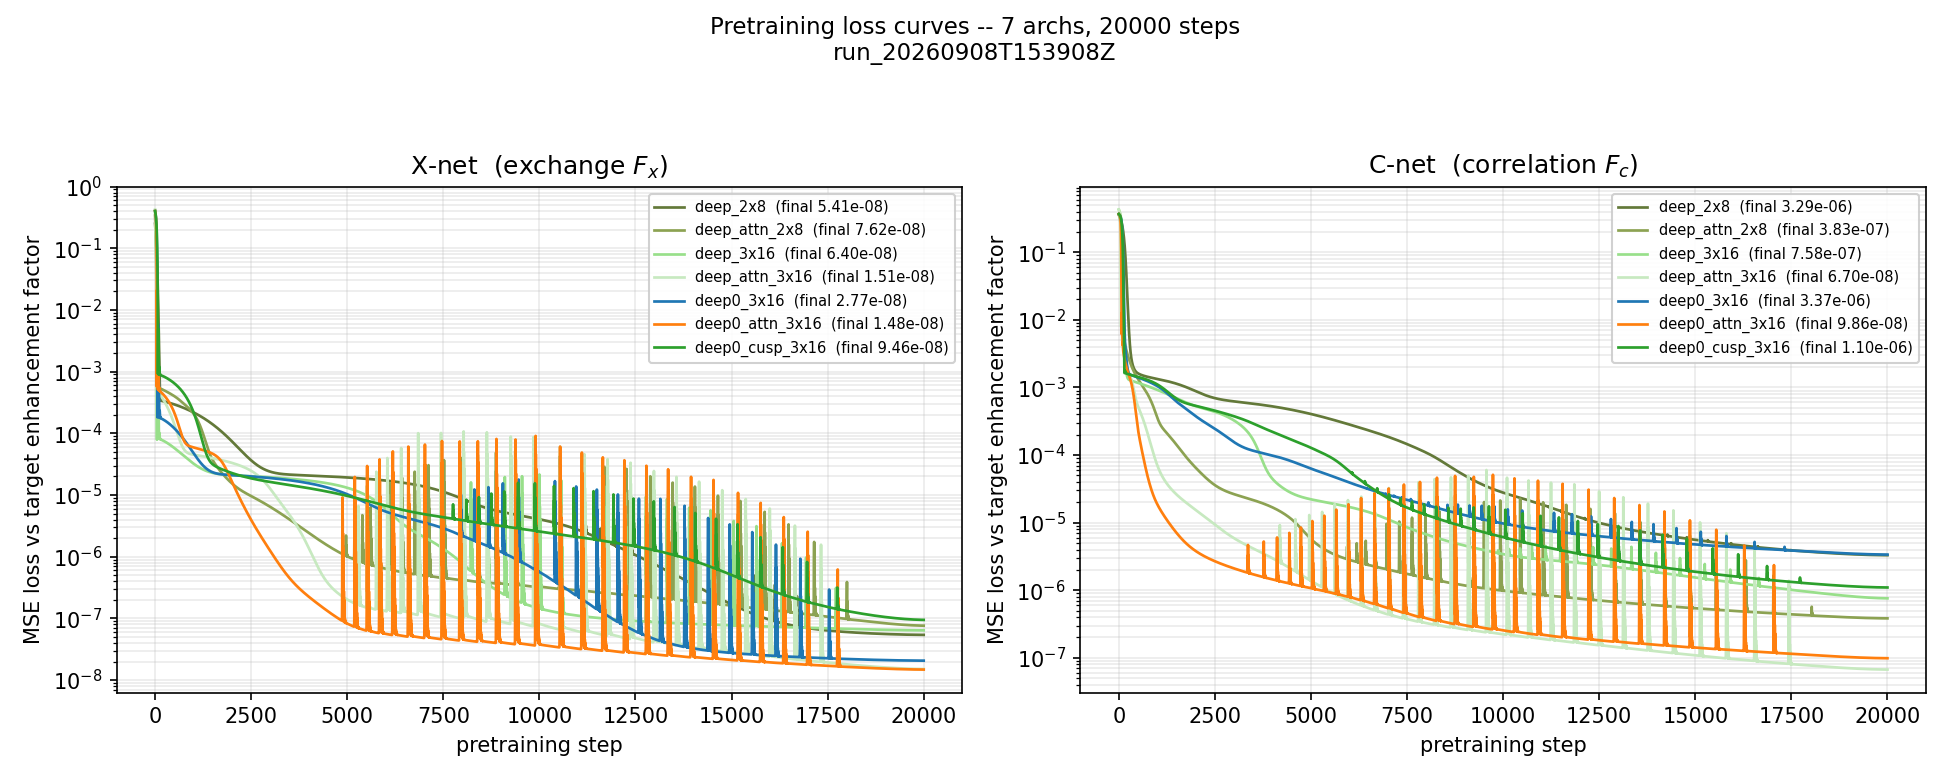
\includegraphics[width=\linewidth]{figures_dfs_step7_v7_family_pretrain/pretrain_curves.png}
  \end{column}
  \begin{column}{0.5\linewidth}
    
\includegraphics[width=\linewidth]{figures_dfs_step7_v7_family_pretrain/uncertified_mgga/pretrain_curves.png}
  \end{column}
  \end{columns}
  \footnotesize
  \begin{itemize}
    \item Pointwise residual per step, exchange (left panel of each pair) and correlation (right); left the seven certified GGA clones, right the four SCAN clones. The recurring bursts from step 4000 to 8000 on are a property of the fit, not of the validation, which reloads nothing.
    \item The GGA clones end at $10^{-8}$ to $10^{-6}$; deep\_attn\_3x16 descends earliest and lowest, at the longest fit (28 h against 3.8 h for its plain twin). The SCAN clones stop 40 to 400 times higher in exchange and fail the certificate.
  \end{itemize}
\end{frame}
\slidenote{Left: the seven certified GGA clones of the size and families runs on one panel pair; right: the four meta-GGA clones whose fits completed (their certificates failed, so they are drawn from their run). The curves are the first term of the pre-training objective, the weighted mean squared pointwise residual, for the exchange network (left panel of each pair) and the correlation network (right panel), against the optimizer step on a log scale; the final value of each curve is in the legend. The regular spikes are bursts of 5 to 14 consecutive steps at 6 to 12 times the local level, recurring every 420 to 590 steps from step 4000 to 8000 onward (the fit decides where) and ending near step 17500; they do not sit on the 50-step validation grid, and no snapshot is reloaded during a fit (the best model is kept aside while training continues from the current weights), so their cause lies in the optimization itself and is not established here. The GGA clones all reach residuals of $1.5\times10^{-8}$ to $9.5\times10^{-8}$ (exchange) and $6.7\times10^{-8}$ to $3.4\times10^{-6}$ (correlation) in units of the squared enhancement-factor difference, which corresponds to sub-kcal/mol atomization errors (previous slides). The attention variants take much longer per step (28 h against 3.8 h) but reach the lowest residuals. The SCAN clones' curves are smooth and still decreasing slowly at 20000 steps; none diverges, they are simply far from converged to SCAN's accuracy, which is consistent with the meta-GGA form (an additional input, $x_\alpha$, and SCAN's more structured dependence on $\alpha$) needing more capacity or more steps than the GGA clones; the lever study of Sec. 6 tests the width and the energy-term weight.}

\begin{frame}{3. Pre-training: the GGA clones against PBE}
  \begin{columns}[T]
  \begin{column}{0.55\linewidth}
    
\includegraphics[width=\linewidth]{figures_dfs_step7_v7_family_pretrain/pretrain_fx_fc_delta_all.png}
  \end{column}
  \begin{column}{0.45\linewidth}
    \small
    \begin{itemize}
      \item The difference $F^{\rm NN} - F^{\rm PBE}$ of every GGA clone, exchange at $n = 1$ and correlation at $r_s = 2$, along $s$; one curve per architecture.
      \item Within $2.5\times10^{-3}$ for $s < 2.5$ ($10^{-3}$ for the 3x16 clones), at most 0.015 at $s = 6$ (deep\_attn\_2x8 exchange; 0.007 for deep\_3x16); the three zero-init clones within $4.2\times10^{-3}$ everywhere.
      \item The region beyond $s = 3$ is sparsely sampled by the pre-training set and is where the clones drift most; the training of Sec. 4 changes the functionals far more (0.1 to 1) than this.
    \end{itemize}
  \end{column}
  \end{columns}
\end{frame}
\slidenote{These figures show how closely each pre-trained network reproduces its parent along one-dimensional slices of the input space: the exchange enhancement factor as a function of $s$ at unit density, and the correlation factor as a function of $s$ at $r_s = 2$. The figure draws only the differences from PBE, one curve per architecture; the titles printed inside these PNGs read "pretrained corrections", a wording left from the plotting script, whereas the curves are the plain differences $F^{\rm NN} - F^{\rm PBE}$ of networks that were fitted to produce PBE, not to correct it (the correction to PBE is what the training of Sec. 4 produces). For $s$ below 2.5, where most of the energy-weighted grid points lie, every GGA clone is within $4 \times 10^{-3}$ of PBE (in exchange the 3x16 clones within $1.5 \times 10^{-3}$ and deep\_2x8 within $2.5 \times 10^{-3}$); the differences grow beyond $s = 3$, a region the pre-training set samples sparsely, but stay below 0.015 (deep\_attn\_2x8 at $s = 6$; 0.007 for the 3x16 clones).}

\begin{frame}{3. Pre-training: a SCAN clone against SCAN}
  \begin{columns}[T]
  \begin{column}{0.55\linewidth}
    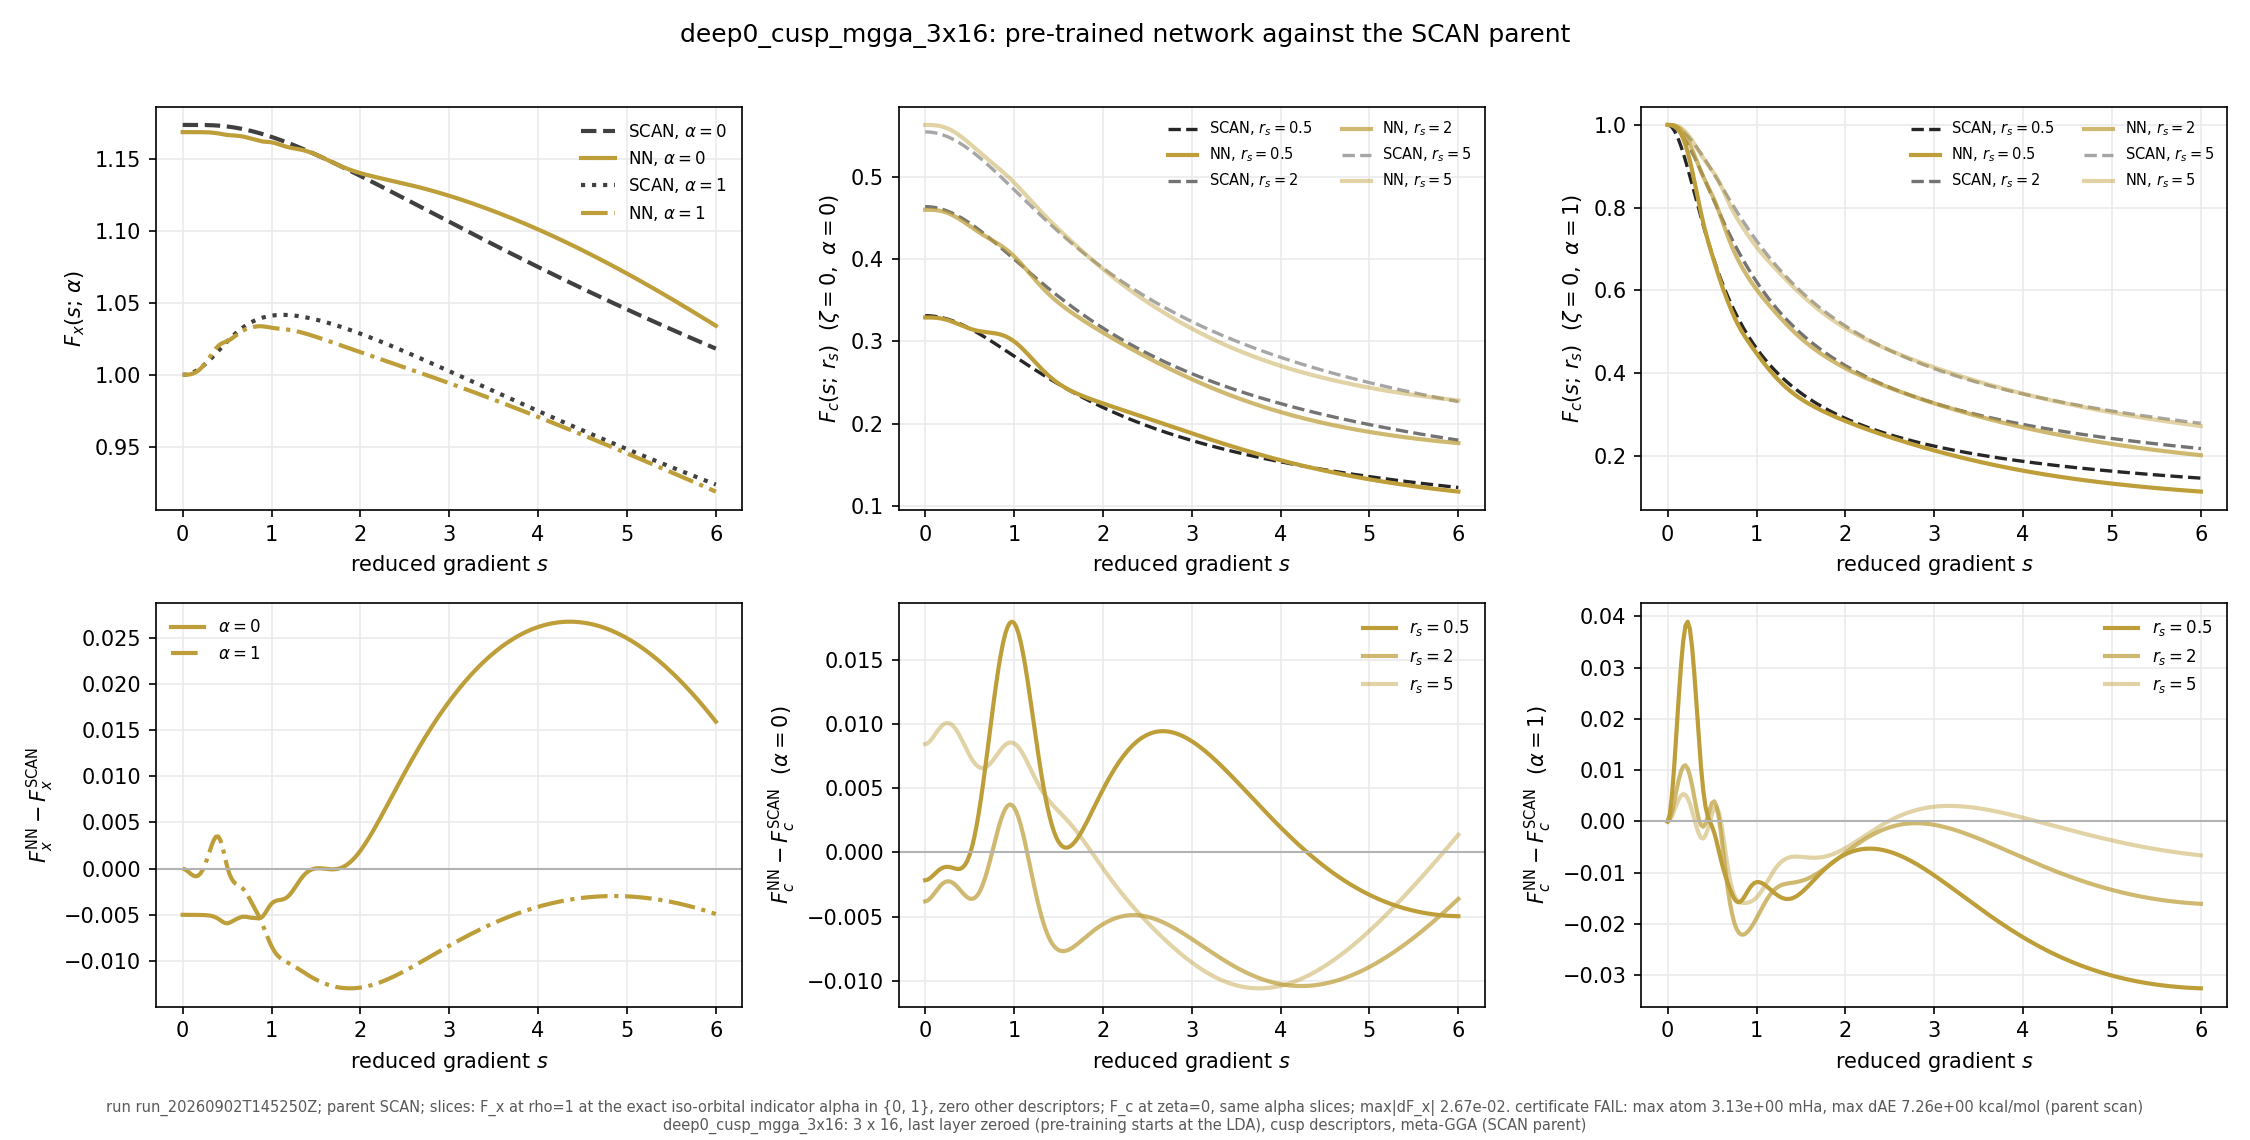
\includegraphics[width=\linewidth]{figures_dfs_step7_v7_family_pretrain/uncertified_mgga/pretrain_fx_fc_deep0_cusp_mgga_3x16.png}
  \end{column}
  \begin{column}{0.45\linewidth}
    \footnotesize
    \begin{itemize}
      \item One of the four SCAN clones (deep0\_cusp\_mgga\_3x16): the parent dashed, the network solid, the difference panels beside them, at $r_s = 0.5$, 2 and 5 and at $\alpha = 0$ and 1.
      \item $F_x(\alpha = 0)$ is 0.01 to 0.027 above SCAN for $s > 2.5$; $F_c(\alpha = 1)$ 0.0003 to 0.016 below it from $s = 2$ at $r_s = 2$ (0.005 to 0.033 at $r_s = 0.5$).
      \item Same-sign offsets over wide $s$ ranges do not cancel between a molecule and its atoms: this is why the clone fails on atomization energies while its pointwise residual is small. The rung-3.5 clones miss SCAN by 0.06 to 0.39 in correlation below $s = 1$; deep0\_mgga\_3x16 sits within 0.01 on every slice and still fails on the atoms.
    \end{itemize}
  \end{column}
  \end{columns}
\end{frame}
\slidenote{The figure is one of the four meta-GGA clones (deep0\_cusp\_mgga\_3x16) against SCAN, along the slices SCAN's paper uses: the enhancement factors against $s$ at three densities ($r_s = 0.5$, 2 and 5) and at the two values of the iso-orbital indicator that mark a single-orbital region ($\alpha = 0$) and a uniform-gas-like region ($\alpha = 1$); the parent is dashed, the network solid, and the difference panels sit below each pair. The clone is above SCAN in exchange at $\alpha = 0$ over a wide range of $s$ and below it in correlation at $\alpha = 1$, and offsets of one sign over wide ranges are exactly what does not cancel in an atomization energy (molecule minus atoms), which is why this clone fails the certificate while its pointwise residual is 40 times the GGA clones' in exchange and 1.5 times in correlation. The other three clones are drawn in the full report (Fig. 3.3): the rung-3.5 clones miss SCAN in correlation by 0.06 to 0.39 below $s = 1$, and deep0\_mgga\_3x16 sits within 0.01 of SCAN on every slice yet fails on the free atoms by 4.1 mHa, so the certificate, computed on the production densities, sees what the slices do not.}

% =====================================================================
\section{4. Optimization, in-sample}

\begin{frame}{4. In-sample: the training objective [DFS21 Eqs. 15--17]}
  \small
  One optimizer step per training group per epoch (a reaction, or a molecule with its density and potential references); the group loss is the DFS weighting ($\lambda_{RE} = 1$, $\lambda_n = 20$), with $E^{\rm NN}$ the self-consistent energy of the $N = 3$ cycle SCF and $t$ the cycle:
  \[
  \mathcal{L} = 1\cdot\mathcal{L}_{AE} + 1\cdot\mathcal{L}_{\rm rxn} + 1\cdot\mathcal{L}_{IP} + 1\cdot\mathcal{L}_{v_{xc}} + 20\cdot\mathcal{L}_{\rho},
  \]
  \[
  \mathcal{L}_{\rm rxn} = \frac{1}{|T|}\sum_{t\in T} w_t^2\, r_t^2, \qquad
  r_t = \sum_i c_i\, E^{\rm NN}_{i,t} - E^{\rm ref}, \qquad
  w_t = \left(\frac{t}{N-1}\right)^2,
  \]
  \[
  \mathcal{L}_{AE} = 0.01\,\mathrm{mean}_Z\, \frac{(E_Z^{\rm NN} - E_Z^{\rm anchor})^2}{(E_Z^{\rm anchor})^2}, \qquad
  \mathcal{L}_{IP} = \mathrm{mean}\,(E^{\rm NN}_{+} - E^{\rm NN}_0 - IP^{\rm ref})^2, \qquad
  \mathcal{L}_{v_{xc}} = \frac{\|V_{xc}^{\rm NN} - V_{xc}^{\rm ref}\|_F^2}{n_{\rm AO}^2},
  \]
  \[
  \mathcal{L}_{\rho} = \mathrm{mean}_{\rm mol}\,\frac{\sum_g w_g\,(n^{\rm NN}_g - n^{\rm ref}_g)^2}{N_e^2}, \qquad N_e = \sum_g w_g\, n^{\rm ref}_g .
  \]
  \begin{itemize}
    \item $\mathcal{L}_{\rm rxn}$ is the DFS convergence-tail scoring ($w_t^2 = 0, 1/16, 1$ at $N = 3$) over the W4-11 atomizations, as reactions with the network's own atoms, and the BH76 barriers [W411, GMTKN55]; the free atoms are held near their exact energies [Chak93]; $V_{xc}$ is compared on the reference density; the density against CCSD on the same grid, per electron. Code: losses.py:76, 366--396; train.py:1829--1835; oneshot.py:632--653.
  \end{itemize}
\end{frame}
\slidenote{This is the actual training step, the only stage that changes the functional away from PBE. \textbf{Group and epoch:} the training data is organized in groups, each a reaction (with its reference energy) or a molecule (with its reference density and potential); one epoch takes one gradient step per group. \textbf{The five channels:} $\mathcal{L}_{\rm rxn}$, the reaction-energy residual: $r_t$ is the reaction energy formed from the network's self-consistent species energies at SCF cycle $t$ (with stoichiometric coefficients $c_i$) minus the reference, and the loss weights the last cycles most (at three cycles the weights are 0, 1/16 and 1), the DFS device that penalizes an SCF that does not settle instead of scoring one arbitrary cycle; the W4-11 atomization energies enter here as reactions "molecule to atoms" using the network's own atomic energies, beside the BH76 barrier heights. $\mathcal{L}_{AE}$, the atom anchors: the free atoms of the subset are held near their exact non-relativistic energies (Chakravorty et al.), as a relative error with the DFS weight 0.01, so that the absolute energy scale is not free to drift. $\mathcal{L}_{IP}$, ionization potentials (cation minus neutral against the reference). $\mathcal{L}_{v_{xc}}$, the exchange-correlation potential matrix compared with a reference potential obtained by inverting the reference density, on the reference density (this channel is not part of the DFS objective); $\|\cdot\|_F$ is the Frobenius norm, the square root of the sum of the squared matrix elements. $\mathcal{L}_\rho$, the density: the squared difference between the network's final SCF density and the CCSD reference density on the same grid, divided by the electron count squared so that molecules of different size weigh alike (DFS Eq. 17). The weights 1 and 20 are the Letter's $\lambda_{RE}$ and $\lambda_n$.}
\codenote{the five channels and their assembly [xcquinox/alec/losses.py:1336--1417]}{slides_code/p21_1_the_five_channels_and_their_assembly.txt}
\codenote{the fixed channel weights 1, 1, 1, 1, 20 [xcquinox/alec/train.py:1829--1835]}{slides_code/p21_2_the_fixed_channel_weights_1_1_1_1_20.txt}
\codenote{the reaction residual (BH76 barriers, W4-11 atomizations as reactions) [xcquinox/alec/losses.py:530--578]}{slides_code/p21_3_the_reaction_residual_bh76_barriers_w4_1.txt}
\codenote{the BH76 channel [xcquinox/alec/losses.py:1282--1310]}{slides_code/p21_4_the_bh76_channel.txt}
\codenote{the ionization channel [xcquinox/alec/losses.py:581--605]}{slides_code/p21_5_the_ionization_channel.txt}
\codenote{the atom anchors: relative squared error at weight 0.01 [xcquinox/alec/losses.py:223--243]}{slides_code/p21_6_the_atom_anchors_relative_squared_error.txt}
\codenote{the atomization channel with the network's own atoms [xcquinox/alec/losses.py:246--273]}{slides_code/p21_7_the_atomization_channel_with_the_network.txt}
\codenote{the potential channel: the Frobenius residual over n\_AO\^{}2 [xcquinox/alec/losses.py:408--483]}{slides_code/p21_8_the_potential_channel_the_frobenius_resi.txt}
\codenote{the density channel per electron [xcquinox/alec/losses.py:366--405]}{slides_code/p21_9_the_density_channel_per_electron.txt}
\codenote{the convergence-tail weights (t/(N-1))\^{}2 [xcquinox/alec/oneshot.py:632--654]}{slides_code/p21_10_the_convergence_tail_weights_t_n_1_2.txt}
\codenote{one optimizer step per training group per epoch [xcquinox/alec/train.py:2001--2061]}{slides_code/p21_11_one_optimizer_step_per_training_group_pe.txt}
\codenote{the group's scoped loss [xcquinox/alec/train.py:1919--1965]}{slides_code/p21_12_the_group_s_scoped_loss.txt}

\begin{frame}{4. In-sample: the training losses (deep\_3x16)}
  \begin{center}
  
\includegraphics[width=\linewidth,height=0.42\textheight,keepaspectratio]{figures_dfs_step7_v7_family_val_best/training_loss_channels_deep_3x16.png}
  \end{center}
  \footnotesize
  \begin{itemize}
    \item SCF: 3 cycles from the converged PBE density, DFS mixing $D_{t+1} = (1 - a_t) D_t + a_t D^{\rm out}_t$, $a_t = 0.3^{t} + 0.3$ [DFS21 SI], gradients through every cycle, the last mixed density scored. AdamW $10^{-3} \to 10^{-5}$ over the second half, weight decay $10^{-4}$, clip 1.0, 200 epochs.
    \item Seven panels, one curve per subset size: the total, the five channels at their trained weights, the validation error at each check. The reaction channel falls in every cell (by 2.3x to 2223x), the density channel by 1.15x to 4.6x, both settled within 25 epochs; the potential channel, absent from the DFS objective, rises in 43 of the 64 cells that carry it, falls in 9 and is flat in 12.
  \end{itemize}
\end{frame}
\slidenote{\textbf{The figure} has seven panels for the deep\_3x16 architecture, one curve per subset size (dark: one point, yellow: twenty-six), each a per-epoch mean on a log scale: the total loss, then the five channels at their trained weights (the five add up to the total), and the validation reaction-energy error at each 25-epoch check with the chosen (validation-best) epoch starred. \textbf{The SCF:} the network's energies and densities are self-consistent, but only three Kohn-Sham cycles are run from the converged PBE density, with the DFS linear mixing schedule (the new density is mixed into the old with a weight $a_t$ that decays from 1.3 toward 0.3); gradients flow through all three cycles. Three cycles are enough when the functional is close to PBE and do not converge when it is far from a fixed point, which is one of the reasons the held-out density comparison is asymmetric (Sec. 5); the 25-cycle arm is the test. \textbf{AdamW} is the optimizer with decoupled weight decay; the learning rate is held for the first half of the run and decayed linearly over the second. \textbf{What the curves show:} the reaction channel is the one the training reduces by orders of magnitude (by 2.3x in the parity arm at 7, trained at weight 0.01, to 188x in deep\_attn\_3x16 at 2 from two points upward, and by 24x to 2223x in the one-point cells); the density channel falls modestly and settles within 25 epochs; the potential channel rises for the larger subsets of the plain networks (deep\_3x16 at 18: 3.9e-5 to 4.3e-5) and falls in every one-point cell and in deep\_attn\_3x16 at 2, 15 and 18, i.e. the potential term and the energy terms pull in different directions once many molecules are supervised.}
\codenote{the SCF: three cycles, the DFS mixing schedule, the tail loss [hpcjobs/configs/dfs\_step7.dfs6311\_grid3\_v7g1\_size.yaml:131--140]}{slides_code/p22_1_the_scf_three_cycles_the_dfs_mixing_sche.txt}
\codenote{the mixing schedule a\_t = 0.3\^{}t + 0.3 [xcquinox/alec/solver.py:303--358]}{slides_code/p22_2_the_mixing_schedule_a_t_0_3_t_0_3.txt}
\codenote{the PBE seed [xcquinox/alec/solver.py:88--125]}{slides_code/p22_3_the_pbe_seed.txt}
\codenote{the SCF cycle: the mixed density scored, gradients through every cycle [xcquinox/alec/solver\_manual.py:404--463]}{slides_code/p22_4_the_scf_cycle_the_mixed_density_scored_g.txt}
\codenote{the cycles as a scan (gradients through every cycle) [xcquinox/alec/solver\_manual.py:263--289]}{slides_code/p22_5_the_cycles_as_a_scan_gradients_through_e.txt}
\codenote{AdamW, the linear decay over the second half, weight decay, the clip [xcquinox/alec/train.py:112--202]}{slides_code/p22_6_adamw_the_linear_decay_over_the_second_h.txt}

\begin{frame}{4. In-sample: validation and the arms' protocol}
  \begin{center}
  
\includegraphics[width=\linewidth,height=0.40\textheight,keepaspectratio]{"figures_dfs_step7_v7_family_val_best/training_loss_channels_deep_3x16 [dpyscf parity].png"}
  \end{center}
  \footnotesize
  \begin{itemize}
    \item Validation MAE on 35 reactions every 25 epochs picks the checkpoint. The 2-to-6-point cells of deep\_3x16, deep0\_3x16 and deep\_2x8 rise after the first check (deep\_3x16 at 2: 11.7 to 32.7 kcal/mol, best at epoch 25); the cells from seven points hold 4.7 to 11.6; the small cells of deep\_attn\_3x16 fall (37 to 7).
    \item The 25-cycle arm keeps everything else and runs 25 SCF cycles, 100 epochs, checks every 10. The parity arm (the figure, with its learning-rate panel) reproduces the DFS code's protocol: 25 cycles, the Letter's weights (reactions 0.01, no potential term), Adam with a plateau schedule at $10^{-4}$ that never triggered.
  \end{itemize}
\end{frame}
\slidenote{The validation error (reactions not in the training subset) separates the cells into two families: the cells trained on 2 to 6 points start overfitting after 25 epochs (their validation error rises), while the one-point cell and every cell from seven points holds 6 to 11 kcal/mol; the validation-best checkpoint is the epoch with the lowest validation error, so the small cells are read at epoch 25. The attention cells behave differently: the small cells of deep\_attn\_3x16 fall from 37 to 7 kcal/mol, those of deep\_attn\_2x8 fall at 3, 4 and 6 and stay near 29 at 2 and 5. \textbf{The arms:} arm A (25 cycles) changes one thing, the number of self-consistent-field cycles, and keeps the objective, the optimizer and the schedule; it ran 100 epochs with checks every 10 and early-stopped at 70 to 90. Arm B (dpyscf parity) reproduces the DFS reference code's protocol in every setting the code can express: the density seed mixed with an atomic guess, the mixing schedule as executed, Adam with a plateau learning-rate schedule (a reduction on a plateau of the validation error, which never triggered, so the rate stayed at $10^{-4}$), the Letter's regularization and channel weights (reactions 0.01, the density 20, no potential channel). The figure is the parity arm's own loss figure; it is the one with a learning-rate panel, flat at $10^{-4}$.}
\codenote{the hyperparameters of the run (200 epochs, 1e-3 to 1e-5, weight decay 1e-4, clip 1.0, validation every 25) [hpcjobs/configs/dfs\_step7.dfs6311\_grid3\_v7g1\_size.yaml:153--183]}{slides_code/p23_1_the_hyperparameters_of_the_run_200_epoch.txt}
\codenote{the validation slice [xcquinox/alec/train.py:745--817]}{slides_code/p23_2_the_validation_slice.txt}
\codenote{the validation reaction-energy MAE [xcquinox/alec/train.py:820--862]}{slides_code/p23_3_the_validation_reaction_energy_mae.txt}
\codenote{the validation-best tracker [xcquinox/alec/train.py:682--742]}{slides_code/p23_4_the_validation_best_tracker.txt}
\codenote{the validation-best checkpoint among the three saved [xcquinox/alec/train.py:1017--1052]}{slides_code/p23_5_the_validation_best_checkpoint_among_the.txt}

\begin{frame}{4. In-sample: the trained enhancement factors, the 3x16 networks}
  \begin{columns}[T]
  \begin{column}{0.5\linewidth}
    
\includegraphics[width=0.84\linewidth]{figures_dfs_step7_v7_family_val_best/trained_fx_fc_deep_3x16.png}
  \end{column}
  \begin{column}{0.5\linewidth}
    
\includegraphics[width=0.84\linewidth]{figures_dfs_step7_v7_family_val_best/trained_fx_fc_deep_attn_3x16.png}
  \end{column}
  \end{columns}
  \footnotesize
  \begin{itemize}
    \item Exchange: the trained $F_x$ is below PBE by 0.002 to 0.06 near $s = 0.8$ and above it from $s = 1.0$ to 1.7, by up to 0.18 (deep\_3x16) and 0.13 (deep\_attn\_3x16) at $s = 1.9$ to 3.4; the one-molecule cell of deep\_3x16 moves least.
    \item Correlation at $r_s = 2$: the one-molecule cells fall to 0.16 by $s = 2$; the others stay near 1 to $s = 2$ (PBE 0.02 by $s = 3$) and then split, deep\_3x16 at 2, 3, 5, 6, 15, 18, 26 decaying to 0.1 to 0.6 by $s = 6$ while 4, 7 and 12 rise to 1.1 to 1.3, and every deep\_attn\_3x16 cell but the one-molecule one rising above 1.
  \end{itemize}
\end{frame}
\slidenote{These are the trained functionals themselves, drawn along the same slices as the pre-training figures: the exchange factor against $s$ at unit density (top left of each figure), its difference from PBE (top right), the correlation factor at $r_s = 2$ (bottom left) and its difference (bottom right), one curve per subset size, at the validation-best checkpoint. Because every cell started from the PBE clone, each curve shows what the training on that subset changed. The exchange change has the same shape in every cell and architecture: a small reduction of $F_x$ at $s$ around 0.8 (the range of most valence density) and a raise between $s = 1.5$ and $s = 6$ (the density tails and the bonding regions), largest for the cells trained on few points (the peak above PBE at $s = 1.9$ to 3.4 is 0.18 for deep\_3x16, 0.13 for deep\_attn\_3x16, 0.14 for deep0\_3x16 and 0.19 for deep0\_attn\_3x16). The correlation change is larger and varies more between cells: PBE's correlation enhancement decays quickly with $s$, while the trained networks keep it near 1 out to $s = 2$ and beyond that either decay slowly or rise above 1 depending on the cell, i.e. the training data at $r_s = 2$ and large $s$ does not determine the correlation factor. The differences from PBE are of order 0.1 to 1, not small perturbations, and the held-out section measures whether they transfer to reactions outside the training subset.}

\begin{frame}{4. In-sample: the trained enhancement factors, the 2x8 pair and the arms}
  \begin{columns}[T]
  \begin{column}{0.5\linewidth}
    
\includegraphics[width=0.84\linewidth]{figures_dfs_step7_v7_family_val_best/trained_fx_fc_deep_2x8.png}
  \end{column}
  \begin{column}{0.5\linewidth}
    
\includegraphics[width=0.84\linewidth]{"figures_dfs_step7_v7_family_val_best/trained_fx_fc_deep_3x16 [25 cycles].png"}
  \end{column}
  \end{columns}
  \footnotesize
  \begin{itemize}
    \item Left, deep\_2x8: the same exchange shape (above PBE by up to 0.08 at $s = 1.9$ to 3.4; deep\_attn\_2x8 by 0.19); in correlation its cells from seven points rise to 1.0 to 1.3 while its small cells decay to 0.2 to 0.4 by $s = 6$.
    \item Right, the 25-cycle arm at 7 and 12: exchange above PBE by up to 0.13, as the parity arm; the parity arm's $F_c$ stays within 0.08 of PBE on every drawn slice (the Letter's weights leave the correlation factor near its start), the 25-cycle arm's within the deep\_3x16 spread.
  \end{itemize}
\end{frame}
\slidenote{The same slices for the remaining architectures on screen: deep\_2x8 (left), the smaller network, whose exchange change has the same shape as the 3x16 networks' at smaller amplitude and whose correlation factor splits the same way between the small subsets (decay) and the subsets from seven points (rise); and the 25-cycle arm (right), the deep\_3x16 network trained under 25 self-consistent-field cycles at 7 and 12 points, whose curves fall inside the spread of the plain deep\_3x16 cells. The attention 2x8 network and the parity arm are drawn in the report: deep\_attn\_2x8 reaches the largest exchange raise of every architecture (0.19), and the parity arm, trained under the Letter's weights with the reaction channel at 0.01, leaves the correlation factor within 0.08 of PBE on every slice (0.10 at $s = 2$ and $r_s = 2$, PBE's own value, where the other cells run up to 1.3), i.e. its training moved the functional least.}

\begin{frame}{4. In-sample: energy and density in DFS units on the training reactions}
  \begin{center}
  
\includegraphics[width=\linewidth,height=0.44\textheight,keepaspectratio]{figures_dfs_step7_v7_family_val_best/insample_by_pool_3x3_eps.png}
  \end{center}
  \footnotesize
  \begin{itemize}
    \item Rows WTMAD-2 / $\varepsilon_n$ / $\mathcal{ED}$, columns BH76 / W4-11 / combined; bars against PBE on each cell's own training reactions (caps), the dashed line PBE on their union (18.6, 3.83, 5.67 kcal/mol).
    \item All 66 trained cells (the two set-aside cells included) are below PBE on $\mathcal{ED}$ over their own reactions: training WTMAD-2 0.00 to 5.4 kcal/mol against 5.67 on the union.
    \item The grid-RMSE density of the trained molecules is below PBE in every cell (NN/PBE 0.57 to 0.97 over the architectures); the per-electron $\varepsilon_n$ of deep\_3x16 is above the pooled PBE value from 2 to 18 points, so the two density measures disagree on the small cells.
  \end{itemize}
\end{frame}
\slidenote{"In-sample" means measured on the very reactions and molecules the cell was trained on: this checks that the training reached what it was asked for, not whether it generalizes. \textbf{The nine panels} use the same layout and metrics as the held-out figure of Sec. 5 (defined there): the top row is the energy error (WTMAD-2), the middle row the density error per electron ($\varepsilon_n$), the bottom row their combination ($\mathcal{ED}$); the columns split the reactions into the BH76 barriers, the W4-11 atomizations, and both together. Each bar is one cell; the black cap over it is PBE on exactly the same reactions; a triangle marks a cell below its cap; the dashed line is PBE on the union of all training reactions of the run. Cells whose subset has no reaction of a column (the one-point cell has no barrier; the three-point subset has no atomization) have no bar there. \textbf{Reading:} every cell reproduces its own training reactions far better than PBE (deep\_attn\_3x16 0.05 to 2.45 kcal/mol, deep0\_attn\_3x16 0.05 to 3.23, the parity arm 4.5 and 5.4), and its training molecules' densities better than PBE in the grid-RMSE measure (NN/PBE 0.72 to 0.97 deep\_3x16, 0.57 to 0.76 deep\_attn\_3x16, 0.68 to 0.93 deep0\_3x16, 0.64 to 0.91 deep0\_attn\_3x16, 0.65 to 0.92 deep\_2x8, 0.71 to 0.86 deep\_attn\_2x8, 0.65 to 0.83 the arms); the per-electron L1 measure $\varepsilon_n$ of the middle row weights the density differently and ranks some small-subset cells above PBE, so the two measures do not agree on the small cells, and both are reported. The in-sample tables count 66 trained cells because the two set-aside cells trained normally; only their held-out passes are refused. \textbf{A panel that is not shown:} the figure suite also produces an in-sample atomization-energy panel that subtracts the network's molecular energy from \textit{fixed, exact} atomic energies rather than from the network's own atoms; that panel measures the network's absolute-energy offset (30 to 110 kcal/mol here), not the trained quantity, and is excluded from every document until it is computed with the network's own atoms.}

% =====================================================================
\section{5. Optimization, hold-out}

\begin{frame}{5. Held-out: the set and the metrics [Goe17; DFS21 Eqs. 20, 21]}
  \small
  Test set: GMTKN55 BH76 barriers and W4-11 atomization energies, minus the 35-reaction validation slice and each cell's training reactions: 61 BH76 rows (three listed twice by name, four more as permuted-name twins; 54 barrier identities are scored) and 120 W4-11 reactions, 189 species with CCSD densities; the tables' n rxn column counts name-deduplicated rows (58 BH76 at one point). PBE is evaluated on each cell's own slice; the functionals with the same 3-cycle SCF they trained with, PBE's density converged.
  \[
  \mathrm{WTMAD\text{-}2} = \frac{56.84}{N}\sum_{i\in\{\rm BH76,\,W4\text{-}11\}} N_i\,\frac{\mathrm{MAD}_i}{\overline{|\Delta E_{\rm ref}|}_i}, \qquad
  \varepsilon_n = \frac{1}{N_e}\int |n - n^{\rm ref}|\, d^3r, \qquad N_e = \int n^{\rm ref}\, d^3r,
  \]
  \[
  \mathcal{ED} = \frac{2}{1/E + 1/(\gamma D)}, \qquad
  D_{\rm RMSE} = \sqrt{\sum_g w_g (n_g - n_g^{\rm ref})^2 \Big/ \sum_g w_g}.
  \]
  \footnotesize
  \begin{itemize}
    \item WTMAD-2 over the two present subsets; alone, a pool reads $56.84\,\mathrm{MAD}_i / \overline{|\Delta E_{\rm ref}|}_i$, a scaled relative error. $\gamma = 1084.87$ kcal/mol on $\varepsilon_n$ (DFS units) or $\gamma = E_{\rm PBE}/D_{\rm PBE}$ on the grid RMSE (self-calibrated).
    \item A cell beats PBE when its $\mathcal{ED}$ is below PBE's on the same slice. Pooled PBE: 8.92 kcal/mol WTMAD-2, $\varepsilon_n$ 0.00923.
    \item The harmonic mean is set by its smaller leg: with $\gamma\varepsilon_n$ at 9.6 to 13.6 kcal/mol here, 1 kcal/mol of $E$ moves $\mathcal{ED}$ by 0.4 to 0.9, the whole density spread by at most 2.7 (1.3 at $E = 8$).
  \end{itemize}
\end{frame}
\slidenote{\textbf{Held-out} means reactions and molecules the cell never trained on. The test set is the union of two standard benchmarks, the BH76 barrier heights and the W4-11 atomization energies (from the GMTKN55 collection), with two removals: 35 reactions set aside as the validation slice used only to pick the checkpoint and the cell's own training reactions; what remains is the cell's "slice" (61 BH76 rows, of which three are listed twice by name and four more are permuted-name twins, so the energy legs average 54 barrier identities), and PBE is scored on the same slice so the comparison is like for like. \textbf{WTMAD-2} is GMTKN55's weighted total mean absolute deviation: each benchmark's mean absolute error is divided by that benchmark's mean absolute reference value (so barriers, around 19 kcal/mol, and atomization energies, around 350 kcal/mol, count as relative errors) and scaled by 56.84 kcal/mol, the mean absolute reference value over all of GMTKN55; here only two of GMTKN55's 55 benchmarks are present, so the figures say "2-subset". $\varepsilon_n$ is the DFS density error: the integrated absolute density difference from the CCSD reference density, per electron (Eq. 20 of the Letter); the grid RMSE is the alternative root-mean-square measure the older figures use. $\mathcal{ED}$ (Eq. 21) combines an energy error and a density error as a harmonic mean, with $\gamma$ converting the density error into kcal/mol: in "DFS units" $\gamma$ is the Letter's published slope 1084.87 and the density leg is $\varepsilon_n$; in "self-calibrated units" $\gamma$ is chosen so that PBE's two legs are equal and the density leg is the RMSE. A harmonic mean is dominated by its smaller term, and since every functional here has a density leg near 10 kcal/mol after $\gamma$, differences in $\mathcal{ED}$ come mostly from the energy leg. "Beats PBE" is defined as a lower $\mathcal{ED}$ than PBE on the same slice.}
\codenote{the full pools (76 BH76, 140 W4-11) before the validation split [xcquinox/alec/full\_benchmark\_pools.py:516--543]}{slides_code/p27_1_the_full_pools_76_bh76_140_w4_11_before.txt}
\codenote{the validation slice, split by reaction identity [xcquinox/alec/eval\_holdout.py:204--245]}{slides_code/p27_2_the_validation_slice_split_by_reaction_i.txt}
\codenote{the strict held-out filter [xcquinox/alec/eval\_holdout.py:173--201]}{slides_code/p27_3_the_strict_held_out_filter.txt}
\codenote{the cell's trained reactions removed [xcquinox/alec/eval\_holdout.py:283--338]}{slides_code/p27_4_the_cell_s_trained_reactions_removed.txt}
\codenote{the energy legs average one term per reaction identity [xcquinox/alec/eval\_holdout.py:402--442]}{slides_code/p27_5_the_energy_legs_average_one_term_per_rea.txt}
\codenote{eps\_n per electron [xcquinox/alec/evaluation.py:196--218]}{slides_code/p27_6_eps_n_per_electron.txt}
\codenote{the grid RMSE [xcquinox/alec/evaluation.py:293--320]}{slides_code/p27_7_the_grid_rmse.txt}
\codenote{WTMAD-2 with the GMTKN55 scale [notebooks/analysis/make\_ablation\_arch\_figure.py:3824--3857]}{slides_code/p27_8_wtmad_2_with_the_gmtkn55_scale.txt}
\codenote{the harmonic mean [notebooks/analysis/make\_ablation\_arch\_figure.py:4835--4841]}{slides_code/p27_9_the_harmonic_mean.txt}
\codenote{the self-calibrated gamma = E\_PBE / D\_PBE [notebooks/analysis/make\_ablation\_arch\_figure.py:4868--4943]}{slides_code/p27_10_the_self_calibrated_gamma_e_pbe_d_pbe.txt}
\codenote{the DFS gamma 1084.87 [notebooks/analysis/make\_ablation\_arch\_figure.py:4952--4975]}{slides_code/p27_11_the_dfs_gamma_1084_87.txt}

\begin{frame}{5. Held-out: energy}
  \begin{center}
  
\includegraphics[width=\linewidth,height=0.42\textheight,keepaspectratio]{figures_dfs_step7_v7_family_val_best/holdout_energy_mae_wtmad2.png}
  \end{center}
  \footnotesize
  \begin{itemize}
    \item Combined WTMAD-2 against subset size, one line per architecture, PBE 8.92 dashed. deep\_3x16 7.92 at one point, 9.61 to 13.97 at two to six, 6.44 to 7.41 from seven to eighteen, 8.23 at twenty-six; deep0\_3x16 (5.90 to 10.48) below PBE at 1, 3, 4 and from seven, above at 2, 5 and 6.
    \item deep\_attn\_3x16 (5.94 to 8.26) and deep\_2x8 (6.18 to 8.85) are below PBE at every cell; deep0\_attn\_3x16 below at 1 and 4 to 12 (6.08 to 8.87), above at 2 and 3; deep\_attn\_2x8 below at 1, 7, 12 and 15, above at 2 to 6 (10.19 to 16.19).
    \item The arms at 7 and 12: 6.92 and 7.17 (25 cycles), 7.44 and 7.48 (parity). The largest subsets (18, 26) do not improve on 7 to 15.
  \end{itemize}
\end{frame}
\slidenote{The energy leg alone: the combined two-subset WTMAD-2 of every cell against the number of training points, with PBE's pooled value as the dashed line; the left panel is the plain mean absolute error, the right the WTMAD-2. deep\_3x16 beats PBE with one training point (H2O alone) and with seven or more, and loses with two to six, as do deep0\_3x16 and deep\_attn\_2x8; deep\_attn\_3x16 beats PBE at every one of its ten cells and deep\_2x8 at every one of its eleven. The one-point result is not an accident of the metric: the cell trained on one molecule changes the functional least. The two-to-six-point cells are the ones whose subsets are barriers and ionizations with almost no atomization energies (Sec. 2), and they overfit (Sec. 4); which property of the subsets causes the loss is not established. The largest subsets (18, 26) do not improve on 7 to 15.}

\begin{frame}{5. Held-out: density}
  \begin{center}
  
\includegraphics[width=\linewidth,height=0.44\textheight,keepaspectratio]{figures_dfs_step7_v7_family_val_best/holdout_density_vs_ccsd.png}
  \end{center}
  \footnotesize
  \begin{itemize}
    \item The held-out density error against CCSD, per cell, beside PBE's on the same species: in the per-electron measure $\varepsilon_n$ (PBE 0.00923) the trained functionals are at or above PBE in every cell but five (deep\_attn\_2x8 at one point, deep\_attn\_3x16 at five, deep0\_attn\_3x16 at one, the parity arm at 7 and 12), by 0.2 to 36 percent.
    \item A fixed set of eight species accounts for the excess (the tail, two slides on); the comparison is asymmetric by protocol: three SCF cycles for the network against a converged PBE density.
  \end{itemize}
\end{frame}
\slidenote{The density leg alone. Each cell's held-out density error is the mean over the 189 held-out species with a CCSD reference density (minus the cell's own training molecules), and PBE's error is computed on the same species, so a cell above the PBE line has, on average, a worse density than PBE where a cell below it has a better one. In the per-electron measure the trained functionals are at PBE's level or above it (worse) in every cell but five; the excess is not spread over the species but concentrated in a fixed handful whose network SCF is farthest from converged after three cycles, which the tail slide shows. The asymmetry by protocol is the caveat that accompanies every density number of this section: the network density comes from three self-consistent-field cycles started from PBE's density and has not converged, while PBE's density is a fully converged calculation.}

\begin{frame}{5. Held-out: energy and density in DFS units (full set)}
  \begin{center}
  
\includegraphics[width=\linewidth,height=0.42\textheight,keepaspectratio]{figures_dfs_step7_v7_family_val_best/holdout_by_pool_3x3_eps.png}
  \end{center}
  \footnotesize
  \begin{itemize}
    \item Rows WTMAD-2 / $\varepsilon_n$ / $\mathcal{ED}$, columns BH76 / W4-11 / combined; the dashed line PBE on the pooled slice, the black cap PBE on each cell's own slice, a triangle a cell below its cap, a star the SCAN comparator where it exists; the $\gamma$ stamp names the units.
    \item $\mathcal{ED}$, 41 of the 64 cells below PBE: deep\_3x16 and deep0\_3x16 at 1, 7, 12, 15, 18, 26 (the two starts agree at every size); deep\_attn\_3x16 at every cell (lowest 7.40 to 7.85 at 4 to 7 points against caps of 9.32 to 9.49); deep0\_attn\_3x16 at 1, 6, 7, 12; deep\_2x8 at 1, 2 and 7 to 26; deep\_attn\_2x8 at 1, 7, 12, 15; both arms at 7 and 12.
    \item The $\mathcal{ED}$ verdict follows the energy verdict in 56 of the 64 cells; in eight (deep\_2x8 at 3 to 6, deep0\_3x16 at 3 and 4, deep0\_attn\_3x16 at 4 and 5) the energy leg is below PBE and the density leg lifts $\mathcal{ED}$ above it.
  \end{itemize}
\end{frame}
\slidenote{The same nine-panel layout as the in-sample figure, now on the held-out slice: rows energy / density / combination, columns barriers / atomizations / both; the greens are deep\_2x8, deep\_attn\_2x8, deep\_3x16 and deep\_attn\_3x16, the greys the two arms, the blue deep0\_3x16, the orange deep0\_attn\_3x16; the dashed line is PBE on the pooled slice and the black cap PBE on each cell's own slice; a triangle marks a cell below its cap; a star marks the SCAN comparator on the panels where SCAN was evaluated; the stamp in the corner names $\gamma$ and the units. \textbf{Combination:} the $\mathcal{ED}$ verdict follows the energy verdict in 56 of the 64 cells (49 cells are below PBE on the energy leg, 41 on $\mathcal{ED}$; the eight that differ have a density leg far enough above PBE's to lift the combination): deep\_3x16 and deep0\_3x16 below PBE at 1, 7, 12, 15, 18 and 26 points, deep\_attn\_3x16 everywhere, deep\_2x8 at 1, 2 and from 7, deep\_attn\_2x8 and deep0\_attn\_3x16 at their small-energy cells, both arms at 7 and 12: 41 of the 64 cells.}

\begin{frame}{5. Held-out: the full set beside the set without the recurring density tail}
  \begin{columns}[T]
  \begin{column}{0.5\linewidth}
    
\includegraphics[width=0.8\linewidth]{figures_dfs_step7_v7_family_val_best/holdout_by_pool_3x3_eps.png}
  \end{column}
  \begin{column}{0.5\linewidth}
    
\includegraphics[width=0.8\linewidth]{figures_dfs_step7_v7_family_val_best_excl_tail/holdout_by_pool_3x3_eps.png}
  \end{column}
  \end{columns}
  \footnotesize
  \begin{itemize}
    \item Left, the full set; right, the same figure with the recurring density tail removed from the density leg: bn (the largest ratio in 55 of the 64 cells), rkt17, cloo, bn3pi, cn, h2, rkt06 and cs, the same eight as before this pull.
    \item Without them the deep\_3x16 column from seven points is within 5 percent of PBE's $\varepsilon_n$ and deep\_attn\_3x16 is below it at 1, 2, 5, 6, 7, 12, 15; the $\mathcal{ED}$ verdicts change only for deep0\_3x16 at three points and deep0\_attn\_3x16 at five. The model-free sibling (38 species with T1 above 0.02 removed) changes the same two cells and deep\_2x8 at three.
    \item The comparison is asymmetric by protocol (an unconverged network density against converged PBE); the converged-SCF re-evaluation (one cell-pass on disk) is the direct test.
  \end{itemize}
\end{frame}
\slidenote{\textbf{Left:} the full set, all eight architecture columns on one axis (the previous slide's figure); deep0\_3x16's combined verdicts match deep\_3x16's at every size (the architecture slide). \textbf{The density tail:} when the per-species density errors are listed, the same handful of species has errors several times PBE's in almost every cell: BN and its $^3\Pi$ state, CN, CS, ClOO, the transition states of OH + Cl (rkt17) and H + CH4 (rkt06), and H2. "Recurring" is the rule that defines the list: a species whose error exceeds 1.5 times PBE's in at least half of the cells that contain it and in at least two. These are multireference or open-shell cases, for which a single-determinant CCSD reference density is itself least reliable, and they are the species whose three-cycle SCF from the PBE seed is farthest from converged (their first-cycle energy step is the largest), so their network density is the least settled. The list is selected by the trained functionals' own errors, so removing it is a diagnostic view, not a model-free one; the model-free list (the 38 species whose CCSD T1 diagnostic exceeds 0.02, six of the eight among them) gives the sibling view, whose verdicts differ from the full set's in three cells. \textbf{Right:} the same cells with those eight species removed from the density leg (the energy leg is unchanged): the density errors of the deep\_3x16 cells from seven points move to within 5 percent of PBE's and several deep\_attn\_3x16 cells go below it, i.e. apart from the tail the trained densities are at PBE's level. The list is unchanged from the 33-cell pull of 2026-09-09, so it is not a property of which cells have landed.}

\begin{frame}{5. The density program: 25 cycles against 3, the same architecture and subsets}
  \begin{center}\small\setlength{\tabcolsep}{4pt}
  \begin{tabular}{llrrrrr}
  \toprule
  Cell & $r$ & WTMAD-2 & $\varepsilon_n$ & grid RMSE & $\mathcal{ED}$ & $\mathcal{ED}$ PBE cap \\ \midrule
  deep\_3x16 & 7 & 6.44 & 0.01017 & 2.39e-04 & 8.13 & 9.49 \\
  deep\_3x16 [25 cycles] & 7 & 6.92 & 0.00972 & 2.20e-04 & 8.36 & 9.49 \\
  deep\_3x16 [dpyscf parity] & 7 & 7.44 & 0.00903 & 2.26e-04 & 8.46 & 9.49 \\
  deep\_3x16 & 12 & 7.41 & 0.01047 & 2.59e-04 & 8.97 & 9.56 \\
  deep\_3x16 [25 cycles] & 12 & 7.17 & 0.00983 & 2.62e-04 & 8.57 & 9.56 \\
  deep\_3x16 [dpyscf parity] & 12 & 7.48 & 0.00892 & 2.29e-04 & 8.44 & 9.56 \\
  PBE & -- & 8.92 & 0.00923 & 2.34e-04 & -- & -- \\
  \bottomrule
  \end{tabular}
  \end{center}
  \small
  \begin{itemize}
    \item Yes on density, modestly: the 25-cycle arm lowers $\varepsilon_n$ by 4.3 percent at 7 and 6.2 percent at 12 and stays above PBE; in the grid RMSE the gain holds at 7 and vanishes at 12 (o3, c2 and fo2 regress). On energy it is a wash and every cell stays under its PBE cap.
    \item The parity arm is the density win: $\varepsilon_n$ 0.00903 and 0.00892, the only deep\_3x16 cells below PBE, bought with a worse energy leg (BH76 WTMAD-2 19.5 against 16.3 and 18.9).
  \end{itemize}
\end{frame}
\slidenote{The table answers the question the density program was set up for: does training with a converged-length self-consistent field (25 cycles instead of 3) improve the density the functional produces on held-out molecules? The rows pair each arm cell with the size-run cell of the same architecture (deep\_3x16) and subset (7 and 12 points); the columns are the combined two-subset WTMAD-2, the per-electron density error, the grid-weighted density RMSE, the combination in DFS units and PBE's combination on the same slice (the cap). The 25-cycle arm improves the per-electron density error in both cells and the grid RMSE in one; its energy leg moves by half a kcal/mol either way. The parity arm, which also runs 25 cycles but under the Letter's channel weights (the reaction channel at 0.01, no potential channel), reaches the lowest density errors of any deep\_3x16 cell and the only ones below PBE's, at the price of a worse barrier-height leg. Both 25-cycle cells stay under PBE's combined cap. The table rows are printed by arm\_vs\_size\_density.py from the two pool CSVs of the figure set.}

\begin{frame}{5. The density program: per species}
  \begin{center}
  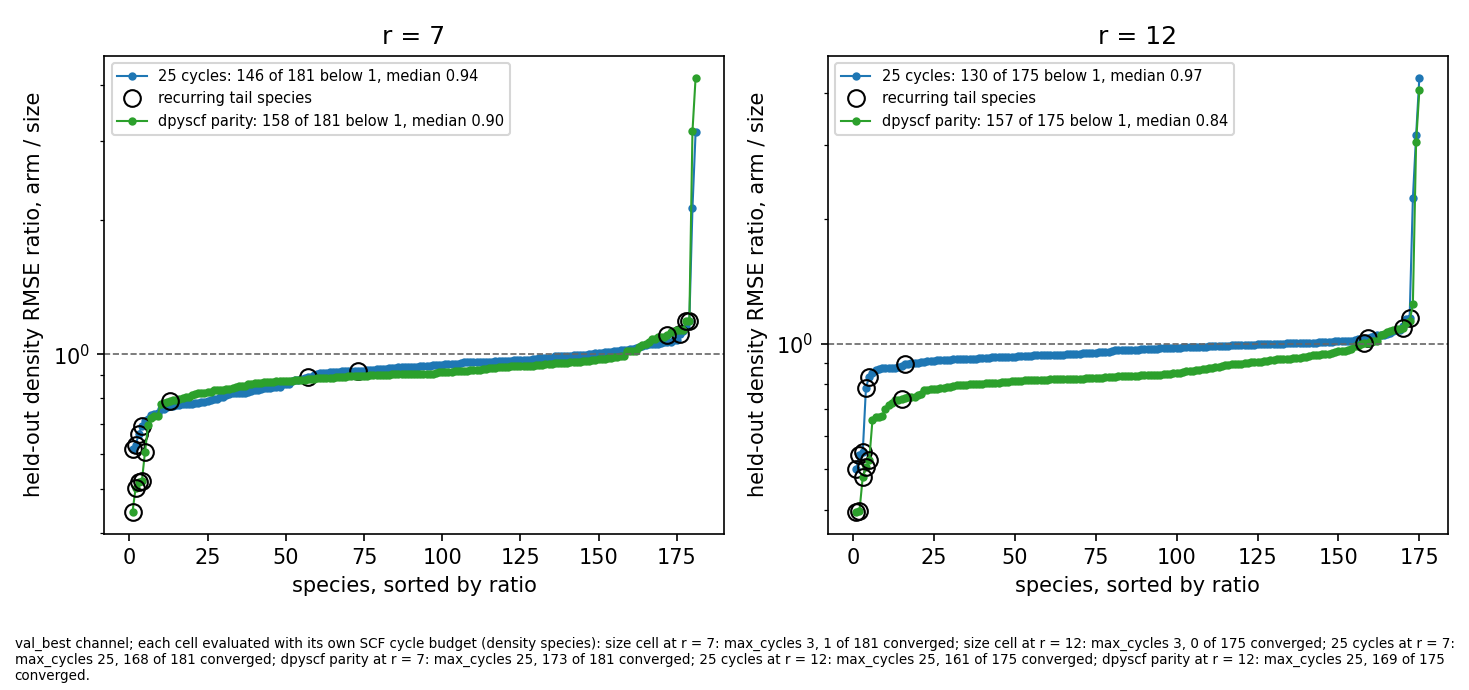
\includegraphics[width=\linewidth,height=0.42\textheight,keepaspectratio]{figures_dfs_step7_v7_family_val_best/arm_vs_size_density.png}
  \end{center}
  \footnotesize
  \begin{itemize}
    \item Per held-out species the ratio of the arm's density RMSE to the size cell's, sorted; below 1 is an improvement. The 25-cycle arm improves 146 of 181 species at 7 (median ratio 0.94) and 130 of 175 at 12 (0.97); the parity arm 158 of 181 (0.90) and 157 of 175 (0.84).
    \item The species helped most (the left ends) are the recurring tail, drawn as hollow markers: part of the tail is the three-cycle evaluation rather than the functionals.
    \item Caveat: the arms were also \emph{evaluated} with 25 cycles (161 to 173 of the species converged) and the size cells with 3 (1 and 0 converged), so training and evaluation protocol are conflated; the converged-SCF re-evaluation of the same networks is the direct test.
  \end{itemize}
\end{frame}
\slidenote{The figure behind the previous table, species by species. For every held-out species the arm's density RMSE against CCSD is divided by the size cell's on the same species; the ratios are sorted and drawn against their rank, one line per arm, on a logarithmic axis, one panel per subset size. A ratio below the dashed line at one is a species the arm reproduces better. The legend states how many species are below one and the median ratio. The hollow markers are the eight recurring tail species; they sit at the left end of every curve, i.e. the extra cycles help most where the three-cycle network density was least settled, which is the reading that part of the tail is the evaluation protocol. The footer states the caveat: the arm cells were evaluated with the 25-cycle budget they were trained with (168 and 173 of 181 species converged at 7, 161 and 169 of 175 at 12), the size cells with the 3-cycle budget (1 and 0 converged), so the comparison mixes a change of training with a change of evaluation; the same networks evaluated under one converged protocol is the test that separates them, and one such cell-pass exists.}

\begin{frame}[label=f34]{5. Held-out: per-cell verdicts, combined leg, DFS units}
  \begin{center}\small
  \begin{tabular}{lll}
  \toprule
  Architecture & Below PBE & At $r$ = \\ \midrule
  deep\_3x16 & 6 of 11 & 1, 7, 12, 15, 18, 26 \\
  deep\_attn\_3x16 & 10 of 10 & every cell \\
  deep0\_3x16 & 6 of 11 & 1, 7, 12, 15, 18, 26 \\
  deep0\_attn\_3x16 & 4 of 8 & 1, 6, 7, 12 \\
  deep\_2x8 & 7 of 11 & 1, 2, 7, 12, 15, 18, 26 \\
  deep\_attn\_2x8 & 4 of 9 & 1, 7, 12, 15 \\
  deep\_3x16 [25 cycles] & 2 of 2 & 7, 12 \\
  deep\_3x16 [dpyscf parity] & 2 of 2 & 7, 12 \\
  \bottomrule
  \end{tabular}
  \end{center}
  \small
  \begin{itemize}
    \item 41 of the 64 cells; the numbers behind every row are on the backup tables. Verdicts within about 10 percent of PBE on a leg depend on the leg and the units: ten cells flip under the plain-MAE leg or the self-calibrated grid-RMSE units, the other 54 carry the same verdict under every choice.
  \end{itemize}
  \hfill \hyperlink{b6}{\beamergotobutton{3x16 table}} \hyperlink{b7}{\beamergotobutton{2x8 and arms}} \hyperlink{b8}{\beamergotobutton{the flips}}
\end{frame}
\slidenote{The verdict of every evaluated cell on the combined leg in DFS units, read from the per-cell table the figure writes (holdout\_by\_pool\_3x3\_eps.csv): a cell is below PBE when its $\mathcal{ED}$ is below PBE's on the same slice. Every deep\_attn\_3x16 cell, deep\_3x16 and deep0\_3x16 at 1 point and at 7 points and above (the same six sizes, the replicate agreement), deep\_2x8 at 1, 2 and from 7, the attention 2x8 and deep0\_attn\_3x16 at their small-energy cells, both arms at 7 and 12: 41 of 64. The verdict of a cell whose $\Delta\mathcal{ED}$ is within a few tenths of zero can change when the energy leg is the plain mean absolute error instead of WTMAD-2 (deep\_2x8 at 3 to 6, deep\_attn\_3x16 at 3, 5 and 6, deep0\_attn\_3x16 at 6), or when the density leg is the grid RMSE with a self-calibrated $\gamma$ instead of $\varepsilon_n$ with the DFS $\gamma$ (deep\_2x8 at 3 to 6, deep\_attn\_3x16 at 2, deep0\_3x16 at 3); the deep\_3x16, deep\_attn\_2x8 and arm verdicts do not depend on those choices. The full rows, with E, $\varepsilon_n$ and $\mathcal{ED}$ for the cell and for PBE, are the two backup tables.}

% =====================================================================
\section{6. Pending}

\begin{frame}{6. Pending: running, queued and set aside}
  \small
  \begin{itemize}
    \item Cells running or queued: deep\_attn\_3x16 at 26 (stopped by the 48 h wall, relaunched from its resume checkpoint), deep\_attn\_2x8 at 26, deep0\_attn\_3x16 at 15 to 26, deep0\_cusp\_3x16 at every subset, the arms at 15 to 26.
    \item Two evaluated cells (deep\_attn\_2x8 at 18, deep\_3x16 [25 cycles] at 15) await re-evaluation: their passes ran while the T1 backfill was rewriting the reference files with a key the reference reader did not accept, so every reference was refused and the tables held no reaction.
    \item The corrected reader (the key accepted; an evaluation that reads no species refused instead of written) is committed and is deployed with the re-runs in a later cluster session; every task whose evaluation starts before that deploy writes the same tables.
    \item The figures and tables regenerate from the same suite as cells land, by one entry per run in family\_runs.yaml.
  \end{itemize}
\end{frame}
\slidenote{\textbf{Running and queued cells:} the remaining columns of the size and families runs are on the cluster, as are the arms' larger subsets (their cells carry the tags [25 cycles] and [dpyscf parity] on the same axis); the figures and tables regenerate from the same suite as they land, by one entry per run in family\_runs.yaml. \textbf{The two cells awaiting re-evaluation:} the CCSD T1 backfill adds one key to every benchmark reference file, and the held-out evaluation's reference reader refused any file carrying a key it did not list; the two evaluations that ran while the files were being rewritten refused every reference, evaluated the network on no species and wrote tables of null values with the task exiting normally, which the figure suite would read as evaluated cells. The reader now lists the key; a reference file the reader cannot read stops the pass with the reason, and an evaluation whose precompute produced no species is refused before any table is written. That code is committed and not yet on the cluster: every task whose evaluation starts before it is deployed writes the same tables, and the deploy and the re-runs are one later cluster session.}

\begin{frame}{6. Pending: the open decisions}
  \small
  \begin{itemize}
    \item Meta-GGA group: four certificates FAIL, one fit cancelled; the training array is held. Landed follow-up: three wider architectures (3x32, 4x16, 4x32) registered and a lever study (fourteen 10000-step fits: energy-term weight 0.1, 10, 100 over the four widths, plus the integration objective on the 3x16) as one 48 h job awaiting submission.
    \item Converged-SCF re-evaluation: one cell-pass (deep\_3x16 at 1, final checkpoint, 214 of 214 converged) took about 13 h of a 24 h job; the campaign at two checkpoints is about 1700 node-hours, so the program's shape is a decision still open. It is the direct test behind the density program's numbers.
    \item The T1 diagnostics landed (203 species, threshold 0.02); the model-free tail-excluded views are rendered from them.
    \item The figure suite's in-sample atomization-energy panel stays out of the documents until it uses the network's own atoms (it now subtracts fixed exact atomic energies and reports the absolute-energy offset).
  \end{itemize}
\end{frame}
\slidenote{\textbf{Meta-GGA:} every completed SCAN clone fails the certificate on the free atoms, so the rung rather than one architecture is what fails at 3x16; the lever study asks whether width or the energy-term weight closes the gap. "Anchored form" means writing the network as SCAN plus a correction rather than the whole factor; it remains one of the options. \textbf{Converged-SCF re-evaluation:} the same trained networks evaluated with a fully converged self-consistent field (DIIS, the direct inversion in the iterative subspace, with the energy converged to $10^{-8}$ Ha) instead of three cycles, which makes the density comparison with PBE symmetric; one cell-pass is on disk and no reading is drawn from it. \textbf{T1 diagnostic:} a standard measure of multireference character from the CCSD amplitudes; the list of species above 0.02 gives the model-free version of the tail-excluded view (Sec. 5). \textbf{The excluded panel:} see the in-sample notes; an atomization energy computed against fixed exact atomic energies measures where the network's absolute energy scale sits, which is not a trained quantity; the panel returns once it is computed against the network's own atoms.}

\begin{frame}{References and sources}
  \scriptsize
  \begin{columns}[T]
  \begin{column}{0.5\linewidth}
  [DFS21] S. Dick and M. Fernandez-Serra, Phys. Rev. B 104, L161109 (2021), with its Supplemental Material; reference code dpyscf.\\[0.3em]
  [PBE96] J. P. Perdew, K. Burke and M. Ernzerhof, Phys. Rev. Lett. 77, 3865 (1996).\\[0.3em]
  [PW92] J. P. Perdew and Y. Wang, Phys. Rev. B 45, 13244 (1992).\\[0.3em]
  [SCAN15] J. Sun, A. Ruzsinszky and J. P. Perdew, Phys. Rev. Lett. 115, 036402 (2015).\\[0.3em]
  [PRSB14] J. P. Perdew, A. Ruzsinszky, J. Sun and K. Burke, J. Chem. Phys. 140, 18A533 (2014).\\[0.3em]
  [OP79] G. L. Oliver and J. P. Perdew, Phys. Rev. A 20, 397 (1979).\\[0.3em]
  [Kato57] T. Kato, Commun. Pure Appl. Math. 10, 151 (1957). \quad [Steiner63] E. Steiner, J. Chem. Phys. 39, 2365 (1963).\\[0.3em]
  [Vas17] A. Vaswani et al., NeurIPS 30 (2017). \quad [Xio20] R. Xiong et al., ICML (2020), arXiv:2002.04745.\\[0.3em]
  [Lin91] J. Lin, IEEE Trans. Inf. Theory 37, 145 (1991).
  \end{column}
  \begin{column}{0.5\linewidth}
  [Goe17] L. Goerigk et al., Phys. Chem. Chem. Phys. 19, 32184 (2017) (GMTKN55, WTMAD-2, BH76RC).\\[0.3em]
  [W411] A. Karton, S. Daon and J. M. L. Martin, Chem. Phys. Lett. 510, 165 (2011).\\[0.3em]
  [HK12] R. Haunschild and W. Klopper, J. Chem. Phys. 136, 164102 (2012).\\[0.3em]
  [Chak93] S. J. Chakravorty et al., Phys. Rev. A 47, 3649 (1993). \quad [NIST] NIST Chemistry WebBook ionization energies.\\[0.3em]
  [code] the repository: \path{xcquinox/alec/networks.py}, \path{descriptors.py}, \path{metagga.py}, \path{config.py}, \path{xcquinox/net.py}, \path{xcquinox/alec/subset_selection.py}, \path{dfs_pool.py}, \path{training_points.py}, \path{pretrain.py}, \path{cluster/fidelity.py}, \path{cluster/grid_config.py}, \path{losses.py}, \path{train.py}, \path{oneshot.py}, \path{solver.py}, \path{evaluation.py}, \path{notebooks/analysis/make_ablation_arch_figure.py}, \path{arm_vs_size_density.py}; the figures and CSVs under \path{notebooks/analysis/figures_dfs_step7_*}; [cfg] the run configurations \path{hpcjobs/configs/dfs_step7.dfs6311_grid3_v7*.yaml}.
  \end{column}
  \end{columns}
\end{frame}
\slidenote{The bracketed keys throughout the deck resolve here. Equations are cited to the paper that defines them and to the repository line that implements them; values are cited to the CSV or run file they are read from; protocol settings to the run configuration files. The file paths are relative to the repository root. [DFS21] is the Letter whose training set, coordinates, objective and metrics this work follows; [PBE96] and [PW92] the parent functional and the LDA correlation it rests on; [SCAN15] the meta-GGA parent; [PRSB14] the source of the 1.174 exchange ceiling DFS used; [OP79] the spin-scaling relation; [Kato57] and [Steiner63] the cusp conditions behind the cusp descriptors; [Vas17] and [Xio20] the attention block and its pre-layer-norm form; [Lin91] the Jensen-Shannon divergence; [Goe17] the GMTKN55 benchmark collection with the WTMAD-2 measure and the BH76 reaction energies; [W411] the atomization-energy benchmark; [HK12] the G2/97 reference atomization energies; [Chak93] the exact atomic energies of the anchors; [NIST] the ionization potentials.}

% =====================================================================
\section*{Backup}

\begin{frame}[label=b1]{Backup: the runs}
  \begin{center}\scriptsize\setlength{\tabcolsep}{2pt}
  \resizebox{\linewidth}{!}{\begin{tabular}{p{1.9cm}p{5.7cm}p{3.5cm}p{2.8cm}}
  \toprule
  Run & Architectures & Cells done / planned & Run directory \\ \midrule
  size & deep\_3x16, deep\_attn\_3x16, deep\_2x8, deep\_attn\_2x8 & deep\_3x16 11/11, deep\_attn\_3x16 10/11, deep\_2x8 11/11, deep\_attn\_2x8 9/11 & \path{run_20260902T145245Z} \\
  families & deep0\_3x16, deep0\_attn\_3x16, deep0\_cusp\_3x16 & deep0\_3x16 11/11, deep0\_attn\_3x16 8/11, deep0\_cusp\_3x16 0/11 & \path{run_20260902T145247Z} \\
  meta-GGA families & deep0\_cusp\_mgga\_3x16, deep0\_mgga\_3x16, deep0\_mgga\_attn\_3x16, deep0\_rung35\_mgga\_3x16, deep0\_rung35ms\_mgga\_3x16 & 0/55 (four certificates FAIL, one fit cancelled) & \path{run_20260902T145250Z} \\
  25-cycle arm & deep\_3x16 [25 cycles] & 2/5 (7, 12) & \path{run_20260908T153856Z} \\
  dpyscf-parity arm & deep\_3x16 [dpyscf parity] & 2/5 (7, 12) & \path{run_20260908T153908Z} \\
  \bottomrule
  \end{tabular}}
  \end{center}
  \hfill \hyperlink{f4}{\beamerreturnbutton{back to Scope}}
\end{frame}
\slidenote{The five runs of the campaign with their per-architecture cell counts and directories; the counts are the evaluated cells in the figures over the planned cells (11 subset sizes per architecture). The two set-aside cells (deep\_attn\_2x8 at 18, deep\_3x16 [25 cycles] at 15) are not counted as done.}

\begin{frame}[label=b2]{Backup: the eleven architectures}
  \begin{center}\scriptsize\setlength{\tabcolsep}{2pt}
  \resizebox{\linewidth}{!}{\begin{tabular}{llllll}
  \toprule
  Architecture & Last layer & Rung, parent & Hidden & Heads & Extra \\ \midrule
  deep\_2x8 & Glorot & GGA, PBE & 2 x 8 & none & none \\
  deep\_attn\_2x8 & Glorot & GGA, PBE & 2 x 8 & 2 & none \\
  deep\_3x16 & Glorot & GGA, PBE & 3 x 16 & none & none \\
  deep\_attn\_3x16 & Glorot & GGA, PBE & 3 x 16 & 4 & none \\
  deep0\_3x16 & zeroed & GGA, PBE & 3 x 16 & none & none \\
  deep0\_attn\_3x16 & zeroed & GGA, PBE & 3 x 16 & 4 & none \\
  deep0\_cusp\_3x16 & zeroed & GGA, PBE & 3 x 16 & none & cusp \\
  deep0\_mgga\_3x16 (\_attn: 4 heads) & zeroed & meta-GGA, SCAN & 3 x 16 & none & $\alpha$ \\
  deep0\_cusp\_mgga\_3x16 & zeroed & meta-GGA, SCAN & 3 x 16 & none & cusp, $\alpha$ \\
  deep0\_rung35\_mgga\_3x16 (\_ms: multishell) & zeroed & meta-GGA, SCAN & 3 x 16 & none & cusp, rung-3.5 occupancy, $\alpha$ \\
  \bottomrule
  \end{tabular}}
  \end{center}
  \scriptsize
  Inputs: $F_x$ from $x_s$, $F_c$ from $x_0, x_1, x_s$; the cusp architectures add $x_4, x_5$ to both, the meta-GGA ones $x_\alpha$ as well, the rung-3.5 ones their occupancy columns (\_ms: one column per shell). The arms' cells carry the run's tag on the same axis: deep\_3x16 [25 cycles], deep\_3x16 [dpyscf parity].

  \hfill \hyperlink{f9}{\beamerreturnbutton{back to the architectures}}
\end{frame}
\slidenote{The registry rows of every architecture the campaign trains or holds: the last-layer start (Glorot or zeroed), the rung and the parent functional the clone reproduces, the hidden layout, the attention heads and the extra descriptors. The rung-3.5 architectures read columns of the localized density matrix in addition to the meta-GGA variables; the multishell variant reads one column per shell.}

\begin{frame}[label=b3]{Backup: the 26-point DFS pool}
  \begin{center}\scriptsize\setlength{\tabcolsep}{2pt}\renewcommand{\arraystretch}{0.78}
  \resizebox{\linewidth}{!}{\begin{tabular}{llp{3.5cm}|llp{5.6cm}}
  \toprule
  Idx & Point & Species (name, charge, spin) & Idx & Point & Species (name, charge, spin) \\ \midrule
  0 & H2 & H2 (0,0), H (0,1) & 13 & NO2 & NO2 (0,1) \\
  1 & N2 & N2 (0,0) & 14 & HN & HN (0,2), H (0,1) \\
  2 & FLi & FLi (0,0), Li (0,1) & 15 & O3 & O3 (0,0) \\
  3 & CHN & CHN (0,0), H (0,1) & 16 & N2O & N2O (0,0) \\
  4 & CO2 & CO2 (0,0) & 17 & CH3 & CH3 (0,1), H (0,1) \\
  5 & F2 & F2 (0,0) & 18 & CH2 & CH2 (0,2), H (0,1) \\
  6 & C2H2 & C2H2 (0,0), H (0,1) & 19 & H2O & H2O (0,0), H (0,1) \\
  7 & CO & CO (0,0) & 20 & H3N & H3N (0,0), H (0,1) \\
  8 & HLi & HLi (0,0), H (0,1), Li (0,1) & 21 & OH+N2\_to\_H+N2O (BH76) & HO (0,1), N2 (0,0), H (0,1), N2O (0,0) \\
  9 & Na2 & Na2 (0,0) & 22 & OH+CH3\_to\_O+CH4 (BH76) & HO (0,1), CH3 (0,1), O (0,2), CH4 (0,0), H (0,1) \\
  10 & NO & NO (0,1) & 23 & HF+F\_to\_H+F2 (BH76) & HF (0,0), F (0,1), H (0,1), F2 (0,0) \\
  11 & CH & CH (0,1), H (0,1) & 24 & Li\_IP (IP13) & Li (0,1), Li+ (1,0) \\
  12 & HO & HO (0,1), H (0,1) & 25 & C\_IP (IP13) & C (0,2), C+ (1,1) \\
  \bottomrule
  \end{tabular}}
  \end{center}
  \scriptsize
  References: atomization energies [HK12] with H2O and C2H2 from [W411]; reaction energies [Goe17, BH76RC]; ionization potentials [NIST]. Code: dfs\_pool.py, training\_points.py:347--420.
  \hfill \hyperlink{f10}{\beamerreturnbutton{back to the pool}}
\end{frame}
\slidenote{The 26 points of the pool with the species each carries; the charge and spin in parentheses are the species' total charge and the number of unpaired electrons ($2S$). The index is the position in the selection ledger, which the chosen-subsets table lists.}

\begin{frame}[label=b4]{Backup: the eleven chosen subsets}
  \begin{center}\scriptsize\setlength{\tabcolsep}{2pt}
  \begin{tabular}{rp{7.0cm}lllll}
  \toprule
  $r$ & Points (ledger index order) & AE / BH76 / IP & JSD & $\rho^{1/3}$ & $s$ & $\alpha$ \\ \midrule
  1 & H2O & 1 / 0 / 0 & 0.0475 & 0.00109 & 0.03764 & 0.00881 \\
  2 & HLi, OH+N2\_to\_H+N2O & 1 / 1 / 0 & 0.0284 & 0.00015 & 0.02372 & 0.00455 \\
  3 & OH+N2\_to\_H+N2O, OH+CH3\_to\_O+CH4, Li\_IP & 0 / 2 / 1 & 0.0228 & 0.00017 & 0.01995 & 0.00267 \\
  4 & CH2, OH+N2\_to\_H+N2O, OH+CH3\_to\_O+CH4, Li\_IP & 1 / 2 / 1 & 0.0203 & 0.00008 & 0.01801 & 0.00218 \\
  5 & HLi, OH+N2\_to\_H+N2O, OH+CH3\_to\_O+CH4, Li\_IP, C\_IP & 1 / 2 / 2 & 0.0163 & 0.00028 & 0.01418 & 0.00183 \\
  6 & HLi, CH, OH+N2\_to\_H+N2O, OH+CH3\_to\_O+CH4, Li\_IP, C\_IP & 2 / 2 / 2 & 0.0130 & 0.00021 & 0.01120 & 0.00156 \\
  7 & CHN, CO2, HLi, CH, OH+N2\_to\_H+N2O, Li\_IP, C\_IP & 4 / 1 / 2 & 0.0102 & 0.00027 & 0.00877 & 0.00120 \\
  12 & CO2, C2H2, CO, HLi, CH, NO2, CH2, OH+N2\_to\_H+N2O, OH+CH3\_to\_O+CH4, HF+F\_to\_H+F2, Li\_IP, C\_IP & 7 / 3 / 2 & 0.0034 & 0.00004 & 0.00292 & 0.00040 \\
  15 & FLi, CHN, CO2, C2H2, CO, HLi, NO, CH, NO2, CH2, OH+N2\_to\_H+N2O, OH+CH3\_to\_O+CH4, HF+F\_to\_H+F2, Li\_IP, C\_IP & 10 / 3 / 2 & 0.0010 & 0.00007 & 0.00081 & 0.00017 \\
  18 & N2, FLi, CHN, CO2, C2H2, CO, HLi, Na2, NO, CH, NO2, N2O, CH2, OH+N2\_to\_H+N2O, OH+CH3\_to\_O+CH4, HF+F\_to\_H+F2, Li\_IP, C\_IP & 13 / 3 / 2 & 0.0004 & 0.00003 & 0.00028 & 0.00007 \\
  26 & the whole pool & 21 / 3 / 2 & 0 & 0 & 0 & 0 \\
  \bottomrule
  \end{tabular}
  \end{center}
  \hfill \hyperlink{f14}{\beamerreturnbutton{back to the chosen subsets}}
\end{frame}
\slidenote{Every row is the training subset of one column of cells, with the three marginal terms of its divergence; the values are recomputed from the descriptor caches and agree with the ledger to $10^{-9}$.}

\begin{frame}[label=b5]{Backup: the fidelity certificate of every clone}
  \begin{center}\scriptsize
  \resizebox{\linewidth}{!}{\begin{tabular}{lllllll}
  \toprule
  Architecture & Parent & Loss X / C & max atom (mHa) & mean $|\Delta AE|$ & max $|\Delta AE|$ & Verdict \\ \midrule
  deep\_2x8 & PBE & 5.4e-8 / 3.3e-6 & 0.369 & 0.343 & 1.421 (C3H8, C4H6) & PASS \\
  deep\_attn\_2x8 & PBE & 7.6e-8 / 3.8e-7 & 0.201 & 0.131 & 0.573 & PASS \\
  deep\_3x16 & PBE & 6.4e-8 / 7.6e-7 & 0.210 & 0.162 & 0.519 & PASS \\
  deep\_attn\_3x16 & PBE & 1.5e-8 / 6.7e-8 & 0.058 & 0.031 & 0.115 & PASS \\
  deep0\_3x16 & PBE & 2.8e-8 / 3.4e-6 & 0.439 & 0.114 & 0.450 & PASS \\
  deep0\_attn\_3x16 & PBE & 1.5e-8 / 9.9e-8 & 0.123 & 0.042 & 0.149 & PASS \\
  deep0\_cusp\_3x16 & PBE & 9.5e-8 / 1.1e-6 & 0.439 & 0.188 & 1.071 (AlCl3) & PASS \\
  deep0\_mgga\_3x16 & SCAN & 5.6e-6 / 1.6e-5 & 4.106 & 1.473 & 5.605 (11 species) & FAIL \\
  deep0\_cusp\_mgga\_3x16 & SCAN & 3.7e-6 / 5.2e-6 & 3.132 & 2.062 & 7.257 (14 species) & FAIL \\
  deep0\_rung35\_mgga\_3x16 & SCAN & 5.9e-6 / 1.05e-5 & 3.001 & 1.780 & 6.303 (11 species) & FAIL \\
  deep0\_rung35ms\_mgga\_3x16 & SCAN & 3.8e-6 / 1.2e-5 & 2.096 & 0.710 & 3.294 (4 species) & FAIL \\
  \bottomrule
  \end{tabular}}
  \end{center}
  \scriptsize
  The pointwise loss is the final value of the pre-training residual for the exchange (X) and correlation (C) networks; the species in parentheses are the molecules above 1 kcal/mol.

  \hfill \hyperlink{f16}{\beamerreturnbutton{back to the certificate}}
\end{frame}
\slidenote{The certificate table of every clone whose fit completed, with the final pointwise residuals; the tolerances are 1.0 mHa on the free atoms, 1.0 kcal/mol on the mean atomization error and 2.0 kcal/mol on the largest.}

\begin{frame}[label=b6]{Backup: per-cell results, combined leg, DFS units, the 3x16 families [holdout\_by\_pool\_3x3\_eps.csv]}
  \begin{center}\tiny\setlength{\tabcolsep}{2.2pt}
  \begin{tabular}{llrrrrrrr|llrrrrrrr}
  \toprule
  Arch & $r$ & E NN & E PBE & eps NN & eps PBE & ED NN & ED PBE & $\Delta$ED & Arch & $r$ & E NN & E PBE & eps NN & eps PBE & ED NN & ED PBE & $\Delta$ED \\ \midrule
  deep\_3x16 & 1 & 7.92 & 8.92 & 0.00951 & 0.00923 & 8.96 & 9.46 & \textbf{-0.50} & deep\_attn\_3x16 & 18 & 6.72 & 8.92 & 0.00993 & 0.00923 & 8.27 & 9.62 & \textbf{-1.35} \\
  deep\_3x16 & 2 & 9.61 & 8.92 & 0.01071 & 0.00923 & 10.52 & 9.44 & +1.08 & deep0\_3x16 & 1 & 8.18 & 8.92 & 0.00997 & 0.00923 & 9.32 & 9.46 & \textbf{-0.14} \\
  deep\_3x16 & 3 & 10.67 & 8.92 & 0.01068 & 0.00923 & 11.11 & 9.32 & +1.79 & deep0\_3x16 & 2 & 9.16 & 8.92 & 0.01143 & 0.00923 & 10.54 & 9.44 & +1.10 \\
  deep\_3x16 & 4 & 11.06 & 8.92 & 0.01182 & 0.00923 & 11.88 & 9.34 & +2.53 & deep0\_3x16 & 3 & 7.99 & 8.92 & 0.01062 & 0.00923 & 9.44 & 9.32 & +0.12 \\
  deep\_3x16 & 5 & 13.97 & 8.92 & 0.01113 & 0.00923 & 12.96 & 9.32 & +3.64 & deep0\_3x16 & 4 & 8.06 & 8.92 & 0.01160 & 0.00923 & 9.83 & 9.34 & +0.48 \\
  deep\_3x16 & 6 & 13.51 & 8.92 & 0.01091 & 0.00923 & 12.62 & 9.34 & +3.28 & deep0\_3x16 & 5 & 10.48 & 8.92 & 0.01099 & 0.00923 & 11.16 & 9.32 & +1.83 \\
  deep\_3x16 & 7 & 6.44 & 8.92 & 0.01017 & 0.00923 & 8.13 & 9.49 & \textbf{-1.35} & deep0\_3x16 & 6 & 10.40 & 8.92 & 0.01097 & 0.00923 & 11.10 & 9.34 & +1.76 \\
  deep\_3x16 & 12 & 7.41 & 8.92 & 0.01047 & 0.00923 & 8.97 & 9.56 & \textbf{-0.59} & deep0\_3x16 & 7 & 5.90 & 8.92 & 0.01051 & 0.00923 & 7.77 & 9.49 & \textbf{-1.72} \\
  deep\_3x16 & 15 & 6.89 & 8.92 & 0.01004 & 0.00923 & 8.44 & 9.60 & \textbf{-1.16} & deep0\_3x16 & 12 & 7.11 & 8.92 & 0.01058 & 0.00923 & 8.78 & 9.56 & \textbf{-0.78} \\
  deep\_3x16 & 18 & 6.74 & 8.92 & 0.00999 & 0.00923 & 8.31 & 9.62 & \textbf{-1.31} & deep0\_3x16 & 15 & 7.10 & 8.92 & 0.01013 & 0.00923 & 8.63 & 9.60 & \textbf{-0.97} \\
  deep\_3x16 & 26 & 8.23 & 8.92 & 0.00973 & 0.00923 & 9.25 & 9.80 & \textbf{-0.55} & deep0\_3x16 & 18 & 6.82 & 8.92 & 0.00996 & 0.00923 & 8.37 & 9.62 & \textbf{-1.26} \\
  deep\_attn\_3x16 & 1 & 8.26 & 8.92 & 0.00925 & 0.00923 & 9.06 & 9.46 & \textbf{-0.40} & deep0\_3x16 & 26 & 8.52 & 8.92 & 0.00961 & 0.00923 & 9.38 & 9.80 & \textbf{-0.42} \\
  deep\_attn\_3x16 & 2 & 7.87 & 8.92 & 0.00972 & 0.00923 & 9.01 & 9.44 & \textbf{-0.43} & deep0\_attn\_3x16 & 1 & 8.11 & 8.92 & 0.00906 & 0.00923 & 8.89 & 9.46 & \textbf{-0.57} \\
  deep\_attn\_3x16 & 3 & 7.22 & 8.92 & 0.00981 & 0.00923 & 8.60 & 9.32 & \textbf{-0.72} & deep0\_attn\_3x16 & 2 & 13.64 & 8.92 & 0.01168 & 0.00923 & 13.14 & 9.44 & +3.70 \\
  deep\_attn\_3x16 & 4 & 6.09 & 8.92 & 0.01020 & 0.00923 & 7.85 & 9.34 & \textbf{-1.49} & deep0\_attn\_3x16 & 3 & 9.52 & 8.92 & 0.01177 & 0.00923 & 10.91 & 9.32 & +1.59 \\
  deep\_attn\_3x16 & 5 & 6.03 & 8.92 & 0.00883 & 0.00923 & 7.40 & 9.32 & \textbf{-1.92} & deep0\_attn\_3x16 & 4 & 8.87 & 8.92 & 0.01127 & 0.00923 & 10.28 & 9.34 & +0.93 \\
  deep\_attn\_3x16 & 6 & 6.09 & 8.92 & 0.00973 & 0.00923 & 7.73 & 9.34 & \textbf{-1.61} & deep0\_attn\_3x16 & 5 & 7.73 & 8.92 & 0.01134 & 0.00923 & 9.49 & 9.32 & +0.17 \\
  deep\_attn\_3x16 & 7 & 5.94 & 8.92 & 0.00963 & 0.00923 & 7.57 & 9.49 & \textbf{-1.91} & deep0\_attn\_3x16 & 6 & 6.90 & 8.92 & 0.01078 & 0.00923 & 8.68 & 9.34 & \textbf{-0.66} \\
  deep\_attn\_3x16 & 12 & 6.61 & 8.92 & 0.01019 & 0.00923 & 8.27 & 9.56 & \textbf{-1.29} & deep0\_attn\_3x16 & 7 & 6.08 & 8.92 & 0.01126 & 0.00923 & 8.12 & 9.49 & \textbf{-1.37} \\
  deep\_attn\_3x16 & 15 & 6.47 & 8.92 & 0.00956 & 0.00923 & 7.97 & 9.60 & \textbf{-1.63} & deep0\_attn\_3x16 & 12 & 7.34 & 8.92 & 0.01100 & 0.00923 & 9.09 & 9.56 & \textbf{-0.47} \\
  \bottomrule
  \end{tabular}
  \end{center}
  \scriptsize
  E in kcal/mol (2-subset WTMAD-2), eps per electron, ED under $\gamma = 1084.87$ kcal/mol; E PBE and eps PBE are the pooled values, ED PBE the cell-slice value. $\Delta$ED = ED NN $-$ ED PBE: \textbf{bold, negative} marks a cell below PBE (26 of these 40 cells).
  \hfill \hyperlink{f34}{\beamerreturnbutton{back to the verdicts}}
\end{frame}
\slidenote{One row per evaluated cell of the four 3x16 networks, the numbers behind the bar charts, read from the CSV the figure writes. \textbf{E NN / E PBE:} the combined 2-subset WTMAD-2 of the cell and of PBE (the pooled PBE value, the same in every row). \textbf{eps:} $\varepsilon_n$, the per-electron density error, for the cell and for PBE (pooled). \textbf{ED NN / ED PBE:} the combination for the cell and for PBE evaluated on that cell's own slice (which is why ED PBE varies from row to row while E PBE and eps PBE do not: the cell's training reactions are removed from its slice). \textbf{$\Delta$ED} is the cell's combination minus PBE's on the same slice; a negative value, set in bold, is a cell that beats PBE. Twenty-six of these 40 cells do: every deep\_attn\_3x16 cell, deep\_3x16 and deep0\_3x16 at 1 point and at 7 points and above, deep0\_attn\_3x16 at 1, 6, 7 and 12. The deep\_3x16 and deep0\_3x16 rows have the same sign at every shared size, the replicate agreement noted on the architecture slide.}

\begin{frame}[label=b7]{Backup: per-cell results, combined leg, DFS units, the 2x8 pair and the arms [holdout\_by\_pool\_3x3\_eps.csv]}
  \begin{center}\tiny\setlength{\tabcolsep}{2.2pt}
  \resizebox{\linewidth}{!}{\begin{tabular}{llrrrrrrr|llrrrrrrr}
  \toprule
  Arch & $r$ & E NN & E PBE & eps NN & eps PBE & ED NN & ED PBE & $\Delta$ED & Arch & $r$ & E NN & E PBE & eps NN & eps PBE & ED NN & ED PBE & $\Delta$ED \\ \midrule
  deep\_2x8 & 1 & 8.18 & 8.92 & 0.00952 & 0.00923 & 9.13 & 9.46 & \textbf{-0.33} & deep\_attn\_2x8 & 1 & 7.98 & 8.92 & 0.00909 & 0.00923 & 8.82 & 9.46 & \textbf{-0.64} \\
  deep\_2x8 & 2 & 6.65 & 8.92 & 0.01116 & 0.00923 & 8.58 & 9.44 & \textbf{-0.85} & deep\_attn\_2x8 & 2 & 16.19 & 8.92 & 0.01193 & 0.00923 & 14.39 & 9.44 & +4.95 \\
  deep\_2x8 & 3 & 7.92 & 8.92 & 0.01148 & 0.00923 & 9.69 & 9.32 & +0.37 & deep\_attn\_2x8 & 3 & 14.36 & 8.92 & 0.01254 & 0.00923 & 13.97 & 9.32 & +4.65 \\
  deep\_2x8 & 4 & 8.62 & 8.92 & 0.01152 & 0.00923 & 10.20 & 9.34 & +0.86 & deep\_attn\_2x8 & 4 & 10.97 & 8.92 & 0.01156 & 0.00923 & 11.70 & 9.34 & +2.36 \\
  deep\_2x8 & 5 & 8.58 & 8.92 & 0.01128 & 0.00923 & 10.09 & 9.32 & +0.77 & deep\_attn\_2x8 & 5 & 13.99 & 8.92 & 0.01066 & 0.00923 & 12.66 & 9.32 & +3.34 \\
  deep\_2x8 & 6 & 8.85 & 8.92 & 0.01134 & 0.00923 & 10.29 & 9.34 & +0.95 & deep\_attn\_2x8 & 6 & 10.19 & 8.92 & 0.01014 & 0.00923 & 10.58 & 9.34 & +1.24 \\
  deep\_2x8 & 7 & 6.18 & 8.92 & 0.01076 & 0.00923 & 8.08 & 9.49 & \textbf{-1.41} & deep\_attn\_2x8 & 7 & 7.12 & 8.92 & 0.01016 & 0.00923 & 8.65 & 9.49 & \textbf{-0.83} \\
  deep\_2x8 & 12 & 7.03 & 8.92 & 0.01076 & 0.00923 & 8.78 & 9.56 & \textbf{-0.78} & deep\_attn\_2x8 & 12 & 7.57 & 8.92 & 0.01073 & 0.00923 & 9.17 & 9.56 & \textbf{-0.39} \\
  deep\_2x8 & 15 & 6.82 & 8.92 & 0.01050 & 0.00923 & 8.53 & 9.60 & \textbf{-1.07} & deep\_attn\_2x8 & 15 & 7.32 & 8.92 & 0.01028 & 0.00923 & 8.84 & 9.60 & \textbf{-0.76} \\
  deep\_2x8 & 18 & 6.74 & 8.92 & 0.01064 & 0.00923 & 8.51 & 9.62 & \textbf{-1.11} & deep\_3x16 [dpyscf parity] & 7 & 7.44 & 8.92 & 0.00903 & 0.00923 & 8.46 & 9.49 & \textbf{-1.03} \\
  deep\_2x8 & 26 & 7.65 & 8.92 & 0.01015 & 0.00923 & 9.03 & 9.80 & \textbf{-0.77} & deep\_3x16 [dpyscf parity] & 12 & 7.48 & 8.92 & 0.00892 & 0.00923 & 8.44 & 9.56 & \textbf{-1.12} \\
  deep\_3x16 [25 cycles] & 7 & 6.92 & 8.92 & 0.00972 & 0.00923 & 8.36 & 9.49 & \textbf{-1.13} & deep\_3x16 [25 cycles] & 12 & 7.17 & 8.92 & 0.00983 & 0.00923 & 8.57 & 9.56 & \textbf{-0.99} \\
  \bottomrule
  \end{tabular}}
  \end{center}
  \scriptsize
  The same columns; \textbf{bold, negative} marks a cell below PBE: 15 of these 24 cells, 41 of the 64 over the two tables. deep\_2x8 is below PBE at every size but 3 to 6, where its energy leg is within 1.0 kcal/mol of PBE and its density leg 22 to 25 percent above; both arms are below PBE at 7 and 12.
  \hfill \hyperlink{f34}{\beamerreturnbutton{back to the verdicts}}
\end{frame}
\slidenote{The remaining 24 evaluated cells in the same columns: the two 2x8 networks and the two arms of the density program (the tagged deep\_3x16 cells trained under 25 SCF cycles and under the dpyscf-parity protocol). Fifteen of them beat PBE: deep\_2x8 at 1, 2 and from 7 points on, deep\_attn\_2x8 at 1, 7, 12 and 15, and both arms at 7 and 12; with the 26 of the previous table, 41 of the 64 evaluated cells.}

\begin{frame}[label=b8]{Backup: the verdicts that depend on the leg or the units [holdout\_ed\_combined.csv]}
  \begin{center}\small
  \begin{tabular}{lp{8.5cm}}
  \toprule
  Choice & Cells whose verdict flips against the DFS-units, WTMAD-2 verdict \\ \midrule
  plain-MAE energy leg & deep\_2x8 at 3, 4, 5 and 6; deep\_attn\_3x16 at 3, 5 and 6; deep0\_attn\_3x16 at 6 \\
  self-calibrated grid-RMSE units & deep\_2x8 at 3, 4, 5 and 6; deep\_attn\_3x16 at 2; deep0\_3x16 at 3 \\
  \bottomrule
  \end{tabular}
  \end{center}
  \small
  Ten cells in all (deep\_2x8 at 3 to 6 flips under both choices); the other 54 of the 64 cells carry the same verdict under every choice, among them every deep\_3x16, deep\_attn\_2x8 and arm cell.
  \hfill \hyperlink{f34}{\beamerreturnbutton{back to the verdicts}}
\end{frame}
\slidenote{The verdict of a cell whose $\Delta\mathcal{ED}$ is within a few tenths of zero can change when the energy leg is the plain mean absolute error instead of WTMAD-2, or when the density leg is the grid RMSE with a self-calibrated $\gamma$ instead of $\varepsilon_n$ with the DFS $\gamma$; the table lists them from the combined-leg CSV of the figure set. The deep\_3x16, deep\_attn\_2x8 and arm verdicts do not depend on those choices.}
